\documentclass{article}
\usepackage{qilin}
\title{ESC195 Notes}
\author{QiLin Xue}
\lhead{ESC195}
\rhead{QiLin Xue}

\begin{document}
    \maketitle
    \tableofcontents
    % \section{Positionality}
\begin{itemize}
    \item A \textbf{position} defines your orientation with respect to an \textbf{entity}.
    \begin{idea}
        How does PIAA affect positionality?
    \end{idea}
    Some ideas from classmates:
    \begin{itemize}
        \item Perception sets initial opinion
        \item You interpret things based on your positionWhat or what you don't perceive affects your positionality.
        \item In breaking the action of perceive-act, you include steps that allow the time to assess your position.
        \item Filters (in perception) depend on position
        \item Understanding your position allows you to assess your interpretations
    \end{itemize}
    \item Subconcious \textbf{bias} will be brought to the table depending on your position, so others can explicityl see how \textit{you} are looking at a situation. 
\end{itemize}
    % \section{Lecture 2}
\begin{itemize}
    \item Numbers are \textit{bases} elements of mathematics, so they cannot be defined explicitly in terms of anything more basic. \item Instead they are defined \textit{implicitly}, by imposing the rules, or \textbf{axioms}, that we require they satisfy.
    \begin{idea}
        The axioms are \textit{inspired} by physical reality, but are not \textit{dictated by it}. They do not exist
    \end{idea}
    \item It is important to have as few axioms as possible (to make it philosophically more ``pure'', and to reduce the risk of contradictions:
    \begin{enumerate}
        \item \textbf{Commutative Law}: For each pair $x,y\in \Re$,
        \begin{equation}
            x+y=y+x
            \label{eq:}
        \end{equation}
        and
        \begin{equation}
            xy=yx
            \label{eq:}
        \end{equation}
        \item \textbf{Associative Law}: For each triple $x,y,z \in\Re$,
        \begin{equation}
            x+(y+z)=(x+y)+z
            \label{eq:}
        \end{equation}
        and
        \begin{equation}
            (xy)z=z(yz)
            \label{eq:}
        \end{equation}
        \item \textbf{Distributive Law} For each triple $x,y,z \in \Re$,
        \begin{equation}
            x(y+z)=zy+yz
            \label{eq:}
        \end{equation}
        and
        \begin{equation}
            (x+y)z=xz+yz
            \label{eq:}
        \end{equation}
        \item \textbf{Existence of Identities}: There exists two distinct real numbers, denoted by $0$ and $1$ for which:
        \begin{equation}
            x+0=0+x=x
        \end{equation}
        and
        \begin{equation}
            x\cdot 1 = 1\cdot x=x
            \label{eq:}
        \end{equation}
        for each $x\in \Re$.
        \item \textbf{Existence of inverses} For each $x \in \Re$, there exists a unique additive inverse which we denote by $-x$ for which
        \begin{equation}
            x+(-x)=(-x)+x=0
            \label{eq:}
        \end{equation}
        For each $x\neq 0$ in $\Re$, there exists a unique multiplactive inverse, which we denote by $x^{-1}$ or $1/x$ for which:
        \begin{equation}
            x\cdot \left(x^{-1}\right) = \left(x^{-1}\right)\cdot x=1.
            \label{eq:}
        \end{equation}
        
        
    \end{enumerate}
    \item It's not important to restrict the number of \textbf{definitions}, which are built from axioms, but it gets messy if we make more definitions that are really needed. (e.g. $4 \equiv 3+1$)
    \begin{definition}
        \textbf{Positive integers} are the ``natural numbers'': $1,2,3,\dots$ Note that:
        $$2 \equiv 1+1$$
        and so forth.
    \end{definition}
    \begin{definition}
        \textbf{Rational numbers} are in the form of:
        $$\frac{a}{b} \equiv a \cdot \frac{1}{b}$$
        where $a$, $b$, are integers are $b \neq 0$. Note that this uses axiom 5 with the definition of fractions to create rational numbers.
    \end{definition}
    \item There is no limit to the number of theorems. We can and should prove all \textit{arithmetic} and \textit{algebraic} theorems rigorously logically, starting from the Axioms (e.g. $4=2+2$).
    \begin{example}
        Let us prove $\sqrt{2}$ is irrational by contradiction. Suppose there is a pair of integers: $a$, $b$, such that:
        $$\left(\frac{a}{b}\right)^2=2$$
        where all common factors have been removed.Therefore:
        \begin{align}
            \therefore\,& a^2=2b^2 \\ 
            \therefore\,&a^2 \equiv 0 \pmod{2} \\ 
            \therefore\,&a \equiv 0 \pmod{2} \\ 
        \end{align}
        We can write $a=2q$ where $q$ is some integer such that:
        \begin{align}
            \therefore\,& a^2=4q^2 \\ 
            \therefore\,& 4q^2 = 2b^2 \\ 
            \therefore\,& b^2 = 2q^2 \\ 
            \therefore\,& b^2 \equiv 0 \pmod{2} \\ 
            \therefore\,& b \equiv 0 \pmod{2}
        \end{align}
        However, since $a$ and $b$ are both even, we have contradicted our statement that all common factors have been removed. Thus $\sqrt{2}$ cannot be rational and can only be irrational.
    \end{example}
    \item However, the 5th field axiom only discusses the creation of rational numbers. We could simply add a ``root 2 axiom'' to create $\sqrt{2}$, just like we did for $0$ and $1$.
    \vspace{2mm}

    \item This is super messy because it would imply we'd need another axiom for every irrational, including every root of every \textbf{polynomial function}:
        \begin{equation}
            P_n(x)=a_nx^n+a_{n-1}x^{n-1}+\cdots+a_1x+a_0
            \label{eq:}
        \end{equation}
    where $a$ can be any specified number and $n$ is a positive integer. If we set $P_n(x)=0$, we get a polynomial equation where we can find the roots.
    \begin{definition}
        If $z$ is a root of $p_n(x)$ then $p_n(z)=0$.
    \end{definition}
    There are $n$ roots\footnote{Per the fundamental theorem of algebra, which is beyond the scope of this course}, most are irrational and are called \textbf{algebraic numbers}.
    \item To prevent creating numerous new axioms, we create a new axiom called \textbf{CORA}: Completeness of the Reals Axiom, which tells us that every non-empty set of real numbers that is bounded above has a least upper bound among the real numbers.
    \begin{definition}
        A set of real numbers, $\mathbb{S}$ is bounded above if and only if there exists some number $M$ such that $x \le M$ for all $x \in \mathbb{S}$. For example:
        \begin{equation}
            \mathbb{S}_1=\{1,3,\frac{17}{5},211\}
            \label{eq:}
        \end{equation}
        Here, $M=211$ or $250$, etc. We can write the first upper bound as:
        \begin{equation}
            \mathrm{ub}\mathbb{S}_1=211
            \label{eq:}
        \end{equation}
    \end{definition}
    \begin{definition}
        The least upper bound is the smallest of all the upper bounds. Here:
        \begin{equation}
            \mathrm{lub}\mathbb{S}_1=211
            \label{eq:}
        \end{equation}
    \end{definition}
    \item Note that we \textbf{do not} require that $\mathrm{lub}\mathbb{S} \in \mathbb{S}$ necessarily. For example, if:
    \begin{equation}
        \mathbb{S}_2 = \{x:x^2<2\}
        \label{eq:}
    \end{equation}
    There are several upper bounds in this set, but is there a least upper bound? We may think intuitively it is $\sqrt{2}$, but we have to be careful! We haven't proved it exists yet. \textbf{However,} CORA has \textit{creates} this new number, $\sqrt{2}$, by demanding that it exists.\footnote{However, proving that the lower upper bound is $\sqrt{2}$ is rather tricky and was removed from the supplement.}
    \item Additionally, CORA does the same for all \textbf{algebraic irrationals} and \textbf{transcendental irrationals}. Without CORA, there would be no irrational numbers!
\end{itemize}
    % \section{Integration}
\subsection{Recap of Integration}
\begin{itemize}
    \item The definite integral has the geometric interpretation as the area under the curve $f(x)$ between $x=a$ and $x=b$ and the $x$ axis:
    \begin{equation}
        \int_a^b f(x) \dd{x}
    \end{equation}
    but can be rigorously defined using a Riemann sum:
    \begin{equation}
        \int_a^b f(x) \dd{x} \equiv \lim_{\Vert P \rVert} \sum_{i=1}^n f(x_i^*)\Delta x_i
        \label{eq:}
    \end{equation}
    Often, we have a uniform partition, such that $\Delta x_i = \frac{b-a}{n}$ where $n$ is the number of partitions. And if we choose to use the right hand endpoint, then:
    \begin{equation}
        f(x_i^*) = f(x_i) = f(x_i) = f\left(a+\frac{b-a}{n}i\right)
    \end{equation}
    \begin{example}
        To solve $\int_0^5 x^2 \dd{x}$, we can choose a uniform partition with:
        \begin{equation}
            \Delta x = \frac{5-0}{n} = \frac{5}{n}
        \end{equation}
        and:
        \begin{equation}
            x_i^* = x_i = i\Delta x \implies f(x_i^*)=(i\Delta x)^2 = \left(i\frac{5}{n}\right)^2
        \end{equation}
        The area approximation is:
        \begin{align}
            A \simeq \sum_{i=1}^n \Delta x_i f(x_i^*) &= \sum_{i=1}^n \left(\frac{5}{n}\right)\left(i\frac{5}{n}\right)^2 \\ 
            &= \frac{125}{n^2} \sum_{i=1}^n i^2 = \frac{125}{n^3} \frac{n(n+1)(2n+1)}{6}
        \end{align}
        Taking the limit as $n\to \infty$, we get:
        \begin{equation}
            \int_0^5 x^2 \dd{x} =  \lim_{n\to\infty} \frac{125}{6}\left(2+\frac{2}{n}+\frac{1}{n^2}\right) = \frac{5^3}{3}.
        \end{equation}
    \end{example}
    \begin{example}
        To evaluate $\int_1^2 x^{-2} \dd{x}$, we can choose
        \begin{equation}
            x_i^* = \sqrt{x_{i-1}x_i}
        \end{equation}
        and a uniform partition of:
        \begin{equation}
            \Delta x = \frac{2-1}{n} = \frac{1}{n}
        \end{equation}
        such that:
        \begin{equation}
            x_i = 1+i\Delta x = 1 + \frac{i}{n} = \frac{n+i}{n}
        \end{equation}
        and
        \begin{equation}
            x_{i-1} = \frac{n+i-1}{n}
        \end{equation}
        such that the area is:
        \begin{align*}
            A &\simeq \sum_{i=1}^n \Delta xf(x_i^*) \\ 
            &= \sum_{i=1}^n \frac{1}{n} \left(\frac{1}{x_i^*}\right)^2 \\ 
            &= \sum_{i=1}^n \frac{1}{n} \frac{1}{x_{i-1}x_i} \\ 
            &= \sum_{i=1}^n \frac{1}{n} \frac{n}{n+i-1}\cdot \frac{n}{n+i} \\
            &= \sum_{i=1}^n n \frac{1}{n+i-1} \cdot \frac{1}{n+i} \\ 
            &= \sum_{i=1}^n \left(\frac{1}{n+i-1}-\frac{1}{n+i}\right) \\ 
            &= n\left[\sum_{i=1}^n \frac{1}{n+i-1} - \sum_{i=1}^n \frac{1}{n+i}\right] \\ 
            &= n\left[\sum_{i=0}^n \frac{1}{n+i} - \sum_{i=1}^n \frac{1}{n+i}\right] \\ 
            &= n\left[\frac{1}{n}+\frac{1}{n+1}+\frac{1}{n+2}+\cdots+\frac{1}{2n-1}-\frac{1}{n+1}-\frac{1}{n+2}-\cdots-\frac{1}{2n}\right] \\ 
            &=n\left(\frac{1}{n}-\frac{1}{2n}\right) \\ 
            &= 1 - \frac{1}{2} = \frac{1}{2}
        \end{align*}
        The part where we cancel out everything is called a \textbf{telescoping series}. Notice how the area doesn't depend on $n$ so we get the exact area, even if we let $n=1$!.
    \end{example}
    \item We need a better way to do integration, so we can define:
    \begin{equation}
        F(x) \equiv \int_a^x f(t) \dd{t}
    \end{equation}
    such that $F'(x) = f(x)$. This is the definition of the antiderivative. This leads to the fundamental theorem of calculus:
    \begin{equation}
        \int_a^b f(t) \dd{t} = F(h) - F(a)
    \end{equation}
    and the indefinite integral can be written as:
    \begin{equation}
        \int f(x) \dd{x} = G(x) + C
    \end{equation}
    The main problem now becomes trying to \textit{find antiderivatives}, which is much easier than Riemann sums, though still more difficult than calculating derivatives.
\end{itemize}
\subsection{Techniques of Integration}
\begin{itemize}
    \item \textbf{Integration by Parts} attempts to reverse the product rule:
    \begin{equation}
        (fg)' = fg' + f'g
    \end{equation}
    Taking the integral of both sides gives:
    \begin{align}
        f(x)g(x) &= \int f(x)g'(x) \dd{x} + \int f'(x) g(x) \dd{x} \\ 
        \int f(x)g'(x) \dd{x} &= \int f(x) g'(x) \dd{x} = f(x)g(x) - \int f'(x)g(x) \dd{x}
    \end{align}
    If the second integral is easier than the first, then we have made substaintial progress.
    \begin{idea}
        Integration of parts tells us that:
        \begin{equation}
            \int u \dd{v} = uv - \int v \dd{u}
        \end{equation}
    \end{idea}
    \begin{example}
        To solve $\int xe^{2x}$, we can let:
        \begin{align}
            &u=x            &\dd{v} = e^{2x} \dd{x} \\ 
            &\dd{u}=\dd{x} &v=\frac{1}{2}e^{2x} 
        \end{align}
        which gives:
        \begin{align}
            & \frac{1}{2}xe^{2x} - \int \frac{1}{2}e^{2x} \dd{x} \\ 
            &= \frac{1}{2}xe^{2x} - \frac{1}{4}e^{2x} + C
        \end{align}
        We can check:
        \begin{align}
            \frac{d}{dx}\left(\frac{1}{2}xe^{2x}-\frac{1}{4}e^{2x}+C\right) \\ 
            &= xe^{2x} + \frac{1}{2}e^{2x}-\frac{2}{4}e^{2x} \\ 
            &= xe^{2x}
        \end{align}
    \end{example}
    \begin{example}
        To solve $\int x^2\sin(2x) \dd{x}$, we let:
        \begin{align}
            &u=x^2            &\dd{v} = \sin 2x\dd{x} \\ 
            &\dd{u}=2x\dd{x} &v=-\frac{1}{2}\cos(2x) 
        \end{align}
        which gives:
        \begin{equation}
            =-\frac{1}{2}x^2\cos 2x + \int x\cos(2x) \dd{x}
        \end{equation}
        and we can apply integration by parts a second time, if we let:
        \begin{align}
            &u=x            &\dd{v} = \cos 2x\dd{x} \\ 
            &\dd{u}=\dd{x} &v=\frac{1}{2}\sin(2x) 
        \end{align}
        which gives us:
        \begin{align}
            &=-\frac{1}{2}x^2\cos(2x) + \frac{1}{2}x\sin(2x) - \int \frac{1}{2}\sin(2x) \dd{x} \\ 
            &=-\frac{1}{2}x^2\cos(2x)+\frac{1}{2}x\sin(2x) +\frac{1}{4}\cos(2X)+C
        \end{align}
    \end{example}
    \begin{example}
        To solve $I=\int e^{x}\sin x\dd{x}$, we can let:
        \begin{align}
            &u=\sin x            &\dd{v} =e^x\dd{x} \\ 
            &\dd{u}=\cos x\dd{x} &v=e^x
        \end{align}
        to give us:
        \begin{equation}
            = e^x\sin x - \int e^{x}\cos x \dd{x}
        \end{equation}
        We apply integration by parts a second time:
        \begin{align}
            &u=\cos x            &\dd{v} =e^x\dd{x} \\ 
            &\dd{u}=-\sin x\dd{x} &v=e^x
        \end{align}
        to get:
        \begin{align}
            I&=e^x\sin x - e^x\cos x - \underbrace{\int e^x\sin x \dd{x}}_{I} \\ 
            2I &= e^x\left(\sin x - \cos x\right) + C' \\ 
            I &= \frac{1}{2}e^x\left(\sin x - \cos x\right) + C
        \end{align}
        and we are done.
    \end{example}
    \begin{example}
        We can also solve integrals that do not appear to have parts, such as $\int \ln x \dd{x}$. We choose:
        \begin{align}
            &u=\ln x            &\dd{v} =\dd{x} \\ 
            &\dd{u}=\frac{1}{x}\dd{x} &v=x
        \end{align}
        to give us:
        \begin{equation}
            \ln x - \int \dd{x} = x\ln x - x + C
        \end{equation}
    \end{example}
    \item For a definite integral, we can write IBP as:
    \begin{equation}
        f(x)g(x)\Big|^b_a-\int_a^b f'(x)g(x) \dd{x}
    \end{equation}
    \begin{example}
        It is \textit{possible} to apply integration of parts to find the integral of $\int \tan x \dd{x} = \int \frac{\sin x}{\cos x} \dd{x}$. We can let:
        \begin{align}
            &u=\frac{1}{\cos x}=\sec x            &\dd{v} =\sin x\dd{x} \\ 
            &\dd{u}=\sec x\tan x &v=-\cos x
        \end{align}
        this gives us:
        \begin{align}
            \int \tan x \dd{x} &= -\frac{\cos x}{\cos x}+ \int \tan x \dd{x}
        \end{align}
        Notice that we could try to subtract the original integral from both sides and get:
        \begin{equation}
            0 = -1
        \end{equation}
        which is clearly wrong! However, we forgot the constant of integration, so the correct statement would be:
        \begin{equation}
            0 + C' = -1 + C
        \end{equation}
        which does not tell us anything interesting.
    \end{example}
\end{itemize}

    % \section{Lecture 4: Projections}
\begin{itemize}
    \item For two nonzero vectors $\vec{v}$ and $\vec{w}$ such that:
    \begin{equation}
        \vec{v}\cdot\vec{w}=0\implies \cos\theta=0\implies \theta=\frac{\pi}{2}
        \label{eq:}
    \end{equation}
    If $\vec{v}$ and/or $\vec{w}$ is the zero vector,
    \begin{equation}
        \vec{v}\cdot\vec{w}=0
        \label{eq:}
    \end{equation}
    is also true.
    \begin{definition}
        $\vec{v}$ and $\vec{w}$ are orthogonal if and only if $\vec{v}\cdot\vec{w}=0$.
    \end{definition}
    \item Projections are what we use to define points in 2-d and 3-d. For example:
    \begin{center}
        \begin{tikzpicture}
            \draw[->] (0,0) -- (5,0) node[right] {$x$};
            \draw[->] (0,0) -- (0,5) node[right] {$y$};

            \draw[thick,->] (0,0) -- (3,4) node[right] {$(v_1,v_2)$};
            \draw[dotted] (0,4) node[left] {$(0,v_2)$} -- (3,4);
            \draw[dotted] (3,0) node[below] {$(v_1,0)$} -- (3,4);

            \draw[very thick,->] (0,0) -- (1,0) node[midway,below] {$\vec{i}=\begin{bmatrix}
                1\\0
            \end{bmatrix}$};
            \draw[very thick,->] (0,0) -- (0,1) node[midway,left] {$\vec{j}=\begin{bmatrix}
                1\\0
            \end{bmatrix}$};

            \draw[thick,->] (0,0) -- (0,3);
            \draw[thick,->] (0,0) -- (4,0);
        \end{tikzpicture}
    \end{center}
    We can write $\vec{v}=\begin{bmatrix}
        v_1\\v_2
    \end{bmatrix}$ as:
    \begin{align}
        \vec{v} &= v_1\vec{i}+v_2\vec{j} \\ 
        &= v_1\begin{bmatrix}
            1\\0
        \end{bmatrix} + v_2\begin{bmatrix}
            0\\ 1
        \end{bmatrix}
        \\ 
        &= \begin{bmatrix}
            v_1\\v_2
        \end{bmatrix}
    \end{align}
    \item Let's generalize this concept to project one vector $\vec{w}$ on another vector $\vec{v}$
    \begin{center}
        \begin{tikzpicture}
            \draw[thick,->] (0,0) -- (8,2) node[right] {$\vec{v}$};
            \draw[thick,->] (0,0) -- (3,3) node[right] {$\vec{w}$};
            \draw[very thick,->] (0,0) -- (3.53,0.88) node[midway,below] {$\vec{u}$};
            \draw[dotted] (3,3) -- (3.53,0.88);
        \end{tikzpicture}
    \end{center}
    We can say that: $\vec{u}$ is the projection of $\vec{w}$ on $\vec{v}$. Based on the way we have constructed $\vec{u}$ we know it has certain properties:
    \begin{itemize}
        \item $\vec{u}$ is parallel to $\vec{v}$, so it can be expressed as a multiple of $\vec{v}$ such that:
        \begin{equation}
            \vec{u}=c\vec{v}
            \label{eq:}
        \end{equation}
        where $c$ is a scalar.
        \item We can say that $\vec{w}-\vec{u}$ (and by extension $\vec{u}-\vec{w}$) is orthogonal to $\vec{v}$:
        \begin{equation}
            (\vec{w}-\vec{u})\cdot \vec{v}=0
            \label{eq:}
        \end{equation}
    \end{itemize}
    Using these two properties, we can solve for the unknown $c$:
    \begin{align}
        (\vec{w}-\vec{u})\cdot \vec{v} &= 0 \\
        \vec{w}\cdot\vec{v}-\vec{u}\cdot\vec{v} &= 0 \\
        \vec{w}\cdot\vec{v}-(c\vec{v})\cdot\vec{v} &= 0 \\ 
        \vec{w}\cdot\vec{v}-c\left(\vec{v}\cdot\vec{v}\right) = 0 
    \end{align}
    Solving for $c$ gives:
    \begin{equation}
        c=\frac{\vec{w}\cdot\vec{v}}{\vec{v}\cdot\vec{v}}
        \label{eq:}
    \end{equation}
    so we have:
    \begin{equation}
        \boxed{\vec{u}=\frac{\vec{w}\cdot\vec{v}}{\vec{v}\cdot\vec{v}}\vec{v}}
        \label{eq:}
    \end{equation}
    \begin{definition}
        The projection of $\vec{w}$ on $\vec{v}$ can be written as:
        \begin{equation}
            \vec{u}=\text{proj}_{\vec{v}}\vec{w}
            =
            \frac{\vec{w}\cdot\vec{v}}{\vec{v}\cdot\vec{v}}\vec{v}
            = \frac{\vec{w}\cdot\vec{v}}{\lVert \vec{v} \rVert^2} \vec{v}
            = \frac{\vec{w}\cdot\vec{v}}{\lVert \vec{v} \rVert} \frac{1}{\lVert\vec{v}\rVert}\vec{v}
            \label{eq:}
        \end{equation}
        where the last part $\frac{1}{\lVert\vec{v}\rVert}\vec{v}$ is a unit vector pointing in the direction of $\vec{v}$.
    \end{definition}
    \item Suppose we wish to project a vector $\vec{v}$ onto another vector (e.g. z-axis) in three dimensions. \textit{The same formula applies.}
    \item Suppose instead we wish to project $\vec{v}$ on a plane, such as the xy plane? If $\vec{v}=\begin{bmatrix}
        v_1\\v_2\\v_3
    \end{bmatrix}$. Then the projection would be $\begin{bmatrix}
        v_1\\v_2\\0
    \end{bmatrix}$.
\end{itemize}
    % \section{Lecture 5}
\begin{itemize}
    \item There is a linear relationship between the force of a wire and the deformation. The slope was called the stiffness:
    \begin{equation}
        k = \frac{F}{\Delta L}
        \label{eq:}
    \end{equation}
    The problem with this is that the slope would be different for different sizes of the same object, so it didn't reflect a particular object's characteristics.
    \item Young modified this relationship to instead measure the tensile strength $\sigma=F/A$ in terms of the strain $\epsilon=\frac{\Delta L}{L}$, such that:
    \begin{equation}
        E = \frac{\sigma}{\epsilon}
        \label{eq:}
    \end{equation}
    This provides a method to experimentally determine the value of $E$, by loading different weights and measuring the strain for each.
    \item A \textbf{Coupon Test} is the testing of a small representative piece of a material to determine the properties. We do this via the setup below, where we place two indicators a length $L_0$ apart. As we load weight onto the rectangle, the distance between the indicators will change to $L_0+\Delta L$.
    \begin{center}
        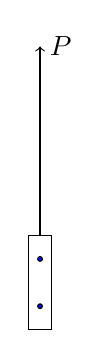
\begin{tikzpicture}[scale=0.3]
            \draw[] (-0.5,2) rectangle (0.5,-2);
            \draw[fill=blue] (0,1) circle (0.1);
            \draw[fill=blue] (0,-1) circle (0.1);
            \draw[->] (0,2) -- (0,10) node[right] {$P$};
        \end{tikzpicture}
    \end{center}
    \item We can increase the strain by adding weights below and measuring the force $P$. Dividing it through by the area gives the tensile strength.
    \begin{center}
        \begin{tikzpicture}
            \coordinate (O) at (0,0);
            \draw[->] (O) -- (12,0) node[above] {$\epsilon$};
            \draw[->] (O) -- (0,6);
            
            \draw[<->,dotted] (0,2.5) -- (3,2.5) node[midway,above] {$\text{linear elastic}$};
            \draw[] (O) -- (3,2);

            \draw[<->, dotted] (3,2.5) -- (6,2.5) node[midway,above] {$\text{yield plateau}$};
            \draw[] (3,2) -- (6,2);
            \draw[dotted] (3,2) -- (0,2) node[left] {$\sigma_{yield}$};
            \draw (0,4) node[left] {$\sigma_{ultimate}$};

            \draw[] (9,4) parabola (6,2);
            \draw[<->, dotted] (6,2.5) -- (9,2.5) node[midway,above] {$\text{strain hardening}$};
            \draw[] (9,4) parabola (11,3);
            \draw[<->, dotted] (9,2.5) -- (11,2.5) node[midway,above] {$\text{necking}$};

        \end{tikzpicture}
    \end{center}
    \item The \textbf{yield plateau} occurs when the atoms in the metal are no longer vibrating back and forth between one another, but sliding across one another. As a result, we experience \textbf{permanent plastic deformations} during this period.
    \item At a certain point, the imperfections build up such that yielding becomes more difficult, so in order to overcome them, the stress increases. This process is known as \textbf{strain hardening}.
    \item \textbf{Necking} occurs after the ultimate stress point where the cable will form a neck shape, reducing the tensile strength.
    \item \textbf{Rupture} occurs after the cable cannot support the strain at all and then break.
    \item If the applied load is taken off, the cable will contract back to $\sigma=0$ following the same slope. After the initial yield plateau, the cable will not be able to naturally go back to its original rest length.
\end{itemize}
    % \section{Lecture Six: Stress-Strain Response}
\begin{itemize}
    \item For a \textbf{brittle} material, the slope of the stress-strain graph will be very high and it will have almost no warning before breaking.
    \begin{itemize}
        \item Applications: Piano wires
    \end{itemize}
    \item Other wires, such as \textbf{flossing wires}, which are used to reinforce concrete, there is a different behaviour, where yielding occurs very early.
    \begin{center}
        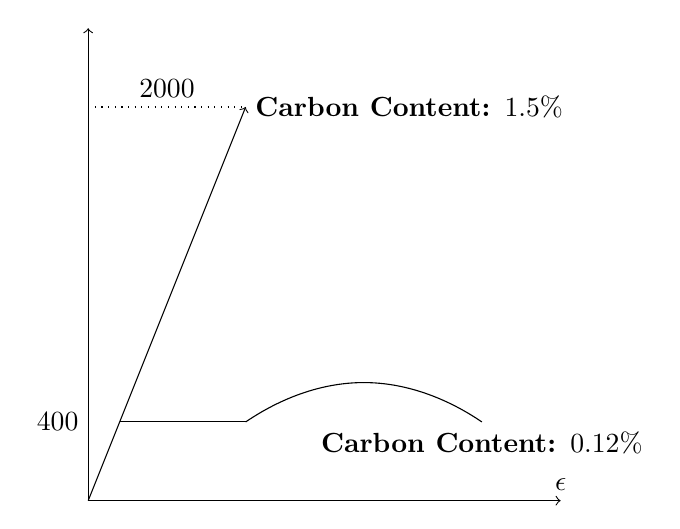
\begin{tikzpicture}
            \coordinate (O) at (0,0);
            \draw[->] (O) -- (6,0) node[above] {$\epsilon$};
            \draw[->] (O) -- (0,6);
            \draw[] (0,1) node[left] {$400\si{\mega\pascal}$};
            \draw[dotted] (0,5) -- (2,5) node[midway,above] {$2000\si{\mega\pascal}$};
            \draw[->] (O) -- (2,5) node[right] {$\textbf{Carbon Content: }1.5\%$};

            \draw[] (0.4,1) -- (2,1);
            \draw[] (3.5,1.5) parabola (2,1);
            \draw[] (3.5,1.5) parabola (5,1) node[below] {$\textbf{Carbon Content: }0.12\%$};
        \end{tikzpicture}
    \end{center}
    \item \textbf{Work} is defined as:
    \begin{equation}
        \text{Work} = \text{Force} \cdot \text{Distance}
        \label{eq:}
    \end{equation}
    and is measured in Joules ($[\si{\joule}]=[\si{\newton\meter}]$) and \textbf{energy} is defined as the capacity to do work
    \item Body fat can store around $40\si{\mega\joule\per\kilogram}$ in body fat, where $7.5\%$ of it can be transferred. One rule of thumb is that one pound of body fat carries you $35$ miles.
    \item Power is the rate at which work is being done. Originally defined as:
    \begin{equation}
        1\text{ HP} = 746\si{\watt}
        \label{eq:}
    \end{equation}
    \item The work, or energy stored in deforming a wire is the area under the curve of the force vs displacement curve. The \textbf{elastic strain energy} gives the maximum recoverable energy, or:
    \begin{equation}
        E=\frac{1}{2}F_\text{max}\Delta_\text{max} = \frac{1}{2}\sigma A \times \epsilon L
        \label{eq:}
    \end{equation}
    The energy density is:
    \begin{equation}
        E/V = \frac{1}{2}\sigma\epsilon
        \label{eq:}
    \end{equation}
    \item The resilience of a material is directly related to its ability to store elastic strain energy.
    \item Some vocabulary terms:
    \begin{itemize}
        \item Weight $[\si{\kilo\newton\per\meter\cubed}]$ - weight density of the material
        \item Stiffness $E[\si{\mega\pascal}]$ - The Young's Modulus: How difficult it is to stretch
        \item Tensile strength $[\si{\mega\pascal}]$- Critical points at which the material starts to yield, or break (ultimate).
        \item Compressive strength  $[\si{\mega\pascal}]$ - yield strength equivalent of tensile strength, except for compressions.
        \item Resilience $[\si{\mega\joule\per\meter\cubed}]$ - maximum energy which a material can absorb per unit volume before experiencing permanent deformations.
        \item Toughness $[\si{\mega\joule\per\meter\cubed}]$ - maximum energy which a material can absorb per unit volume before experiencing permanent deformations.
        \item Ductility is the maximum elongation before it experiences failure.
        \item $\alpha[10^{-6} \si{\per\celsius}]$ - thermal expansion coefficient
    \end{itemize}
\end{itemize}
    % \section{Technical Mechanical Behaviour}
\begin{itemize}
    \item The ultimate tensile strength, denoted as $UTS$ or $\sigma_\text{UTS}$ is the highest stress that a material can occur in a material.
    \item The \textit{proportional limit} describes the point on the tensile stress-strain curve where elastic deformations no longer occur.
    \item Along with the yield strength, it is difficult to define this objectively. Instead, we use the following convention:
    \begin{definition}
        The yield strength is the stress value at which if the material is unloaded at that point, the strain will be $\epsilon = 0.002 = 0.2\%$.
    \end{definition}
    \item Uniform deformation occurs when the thickness of the material is uniform. Non-uniform deformation occurs when an increase in strain results in a decrease in stress. This is known as \textbf{necking}.
\end{itemize}
    % \section{Polymers}
\begin{itemize}
    \item A useful analogy for polymers is to imagine a \textit{molecular hand}. A polymer is consisted of several twisted and tangled chains of molecules. This is known as \textit{entanglement}. This is due to the non-linear nature of the polymers and the fact that bonds can rotate.
    \item To plastically deform a polymer, we can imagine a microscopic hand pulling a polymer. If you are able to do so, then it is seen as plastic deformation
    \item The molecular chains are connected via weak intermolecular forces. Increasing the temperature increases the vibration, allowing the molecular hand to more easily separate them.
    \begin{idea}
        When a polymer undergoes a physical transformation (i.e. melting, dissolving, deforming), it is due to the intermolecular interactions, not the intramolecular interactions. 
    \end{idea}
    \begin{case}
        Plastic exhibits very interesting behaviour when it is stretched. During plastic deformation, the molecules can line up, which can cause the following physical changes:
        \begin{itemize}
            \item Color change (lighter)
            \item Strong in the direction of stretching
            \item Weaker in the direction perpendicular to stretching
        \end{itemize}
        The polymers become \textit{oriented} (also known as \textit{conditioned}) with the loading axis. This is a great demonstration that shows how polymers can be thought of as an interconnected mix of long polymer chains.
    \end{case}
    \item We define the yield strength as the point in which necking occurs (first local maximum in the stress-strain curve)
    \subsection{Chemical Basics}
    \item To describe the polymers on a molecular level, we look at it from an organic chemistry perspective. Instead of unit cells, we look at \textit{mer} units (the suffix of \textit{polymer}), which is the starting molecule when building the polymer.
    \begin{case}
        Polyethylene (PE) is a polymer that is consisted of ethene (or more commonly known as ethylene), shown below:
        \begin{center}
            \chemfig{C(-[3]H)(-[5]H) =   C(-[1]H)(-[7]H)}
        \end{center}
        and polyethylene looks like:
        \begin{center}
            \chemfig{-C(-[2]H)(-[6]H)-[@{op,.75}]C(-[2]H)(-[6]H)-C(-[2]H)(-[6]H)-[@{cl,0.25}]C(-[2]H)(-[6]H)-}
            \polymerdelim[height = 5pt, indice = \!\!]{op}{cl}
        \end{center}
        \vspace{2mm} % weird space, don't know why this is the case
        Notice the absence of the double bond. This is due to the chemical reaction that is required to take the mer unit and add it to the polymer.
    \end{case}
    \item Here are some other examples:
    \begin{itemize}
        \item  Polypropylene (PP) is a very common polymer used in many areas (e.g. Starbucks reusable cups). It is a material that is generally stronger and has a higher elastic modulus than polyethylene. This is because it has an extra \ch{CH3} methyl group, as shown below:
        \begin{center}
            \chemfig{-[@{op,.75}]C(-[2]H)(-[6]H)-C(-[2]H)(-[6]CH_3)-[@{cl,0.25}]}
            \polymerdelim[height = 5pt, indice = \!\!]{op}{cl}
        \end{center}
        \item Polyvinylchloride (PVC), along with PE and PP are the three most produced polymers in the world. The structure is similar, except with a chloride atom in the monomer unit:
        \begin{center}
            \chemfig{-[@{op,.75}]C(-[2]H)(-[6]H)-C(-[2]H)(-[6]Cl)-[@{cl,0.25}]}
            \polymerdelim[height = 5pt, indice = \!\!]{op}{cl}
        \end{center}
        The term \textit{vinyl} describes two carbon atoms connected via double bond.
    \begin{case}
        PVC is very strong and has a high elastic modulus. We can explain this by looking at the chemical properties of the chloride atom. Chlorine is an extremely electronegative atom, meaning it tends to attract electrons. This allows it to attract electrons from the hydrogen of neighbouring polymers, forming a hydrogen bond\footnote{Hydrogen bonds are actually much more complicated than this, but this isn't a chemistry course.} This forms a dipole moment, which can be illustrated below via the following notation:
        \vspace{4mm}
        \begin{center}
            \chemfig{
                \chemabove[3pt]{H}{\scriptstyle\delta^+}(-[::270,0.5,,,draw=none]@{c})-
                \chemabove[3pt]{Cl}{\scriptstyle\delta^-}(-[::270,0.5,,,draw=none]@{d})
               }
               \chemmove{
                       \draw[|->] (c)--(d);
               }
        \end{center}
        \vspace{2mm}
        The $\delta^+$ and $\delta^-$ signify the \textit{partial charges} and the arrow is the shorthand notation for the direction of the dipole (which will always point in the direction a proton would move in)
        \vspace{2mm}

        Since this bond is so strong, it is harder for nearby polymers to move against each other due to stronger intermolecular forces. Similarly, PP is strong for similar chemical properties. However instead of hydrogen bonds, it is the extra methyl group increasing london dispersion forces between neighbouring gorups.
    \end{case}
    \item Polytetrafluoroethylene (PTFE) is used for non-stick surfaces. As a result, it is very non-reactive, and it is able to do so due to the large fluorine atoms bonded to each carbon:
    \begin{center}
        \chemfig{-[@{op,.75}]C(-[2]F)(-[6]F)-C(-[2]F)(-[6]F)-[@{cl,0.25}]}
        \polymerdelim[height = 5pt, indice = \!\!]{op}{cl}
    \end{center}
    Their large size helps protect intramolecular bonds within PTFE from being broken and although they are highly electronegative, they are actually nonpolar due to its symmetry.
    \item Polymethylmethacrylate (PMMA) are often used for windows because they can be made optically transparent. The reason they are transparent is because of a bulky side group in their monomer unit that prevents close packing of polymer chains, creating an \textit{amorphous} structure.
    \begin{center}
        \chemfig{-[@{op,.75}]C(-[2]F)(-[6]F)-C(-[2]F)(-[6]C(=[0]O)(-[6]O(-[6]CH_3)))-[@{cl,0.25}]}
        \polymerdelim[height = 5pt, indice = \!\!]{op}{cl}
    \end{center}
    \begin{case}
        We investigate what makes a material transparent, translucent, and opaque from a materials science perspective Polymers can easily align with one another and become organized, which is known as crystallization. When it crystallizes, the index of refraction is different from when it is amorphous. Therefore, if it contains parts that are both amorphous and crystalline (known as \textit{semicrystalline}), the light will not follow a direct path and the polymer will become translucent or opaque.
        \vspace{2mm}

        So how do we make a polymer transparent? If it is completely crystalline, then it would be transparent but polymers can never be 100\% crystalline. Instead, we want them to be 100\% amorphous.
        \vspace{2mm}

        Moving away from the domain of polymers, sapphire has a crystalline structure, made of $Al_2O_3$, and is clear and transparent. Window glass made from silica is amorphous and also clear and transparent. While polycrystalline metals are opaque, we can also have glassy metals, but they are also opaque. To get the full picture, we need a better understanding of how light works.
    \end{case}
    \end{itemize}
    \item To draw bonds going out and in of the page, we use a shaded triangle and dashed triangle, respectively. For example, we would draw methane as:
    \begin{center}
        \chemfig{C(<:[-0.3]H)(<[-1.1]H)(-[2]H)(-[5]H)}
    \end{center}
    \item We often use the symbol $R$ to denote an arbitrary functional group.
    \subsection{Length}
    \item We can characterize the length of a polymer with its linear mass density and the total mass.
    \begin{case}
        Ultrahigh Molecular Weight Polyethylene is often used in hip replacements. It often replaces part of the hip to prevent parts of it from wearing it away. It has high strength, high tolerance, and biocompatible.
        \vspace{2mm}

        As we increase molecular weight in a polymer, we increase the strength and typically increase the strain to fracture due to the increased entanglement of the long molecules.
    \end{case}
    \item The \textbf{number average molecular weight} can be defined as:
    \begin{equation}
        \overline{M}_\text{number} = \sum_{n=1}^i M_nx_n
    \end{equation}
    for a polymer containing $i$ groups where $M_n$ is the molecular weight of the $n^\text{th}$ group and $x_n$ is the number fraction of the $n^\text{th}$ group.
    \item Similarly, the \textbf{weight average molecular weight} can be defined as:
    \begin{equation}
        \overline{M}_\text{weight} = \sum_{n=1}^i M_nw_n
    \end{equation}
    where $w_n$ is the weight fraction of the $n^\text{th}$ group. The weight average will always be larger (and maintains equality) than the number average.
    \begin{proof}
        Suppose we have $i$ groups with molecular weights of $\{M_1, M_2, \dots, M_n\}$ and number fractions of $\{x_1, x_2, \dots \}$. We can calculate the weight fraction to be:
        \begin{equation}
            w_n = \frac{M_nx_n}{M_1x_1+M_2x_2 + \cdots +M_ix_i} = \frac{M_nx_n}{\overline{M}_\text{number}}
        \end{equation}
        so we have:
        \begin{equation}
            \overline{M}_\text{weight} = \frac{1}{\overline{M}_\text{number}}\sum_{n=1}^i  M^2_nx_n
        \end{equation}
        We propose that $\overline{M}_\text{number} \le \overline{M}_\text{weight}$ such that:
        \begin{align}
            \overline{M}_\text{number} & \le  \frac{1}{\overline{M}_\text{number}}\sum_{n=1}^i  M^2_nx_n \\ 
            \overline{M}^2_\text{number} &\le \sum_{n=1}^iM^2_nx_n \\ 
            \sum_{n=1}^i M_nx_n &\le \sqrt{\sum_{n=1}^i M^2_nx_n}
        \end{align}
        The right hand side gives the RMS average and the left hand side gives the arithmetic average. According to the \href{https://en.wikipedia.org/wiki/HM-GM-AM-QM\_inequalities}{RMS-AM inequality}, the RMS mean is always greater or equal to the arithmetic mean.
    \end{proof}
    This \textbf{disparity} is actually quite important, and is also known as the \textbf{polydisperity index} and is defined as:
    \begin{equation}
        \text{\DJ} = \frac{\overline{M}_\text{weight}}{\overline{M}_\text{number}}
    \end{equation}
    \subsection{Close Packing and Crystallization}
    \item As polymer chains line up, the density can increase. Since the chains get closer together, the strength of the intermolecular interactions may also increase, increasing the elastic modulus.
    \item When polymers line up, they form a crystalline structure (i.e. zigzag pattern). However, there will always still be some amorphous sections. As a result, there is an incentive to increase crystallinity and this can be accomplished by having simple mer units and regular repeating structures.
    \item When functional groups are on the same side, such as shown below, it is easier for the polymer to have a close packing behaviour:
    \begin{center}
        \chemfig{[-0.3]-C(<[-1.6]R)(<:[5.6]H)-[0.3]C(<[-1.6]R)(<:[5.6]H)-[-0.3]C(<[-1.6]R)(<:[5.6]H)-[0.3]C(<[-1.6]R)(<:[5.6]H)-[-0.3]}
    \end{center}
    The \textbf{tacticity} describes how the functional groups line up. If they are all on the same side, it is known as \textbf{isotactic}.
    \item If functional groups alternate, it is known as \textbf{syndiotactic}
    \begin{center}
        \chemfig{[-0.3]-C(<[-1.6]R)(<:[5.6]H)-[0.3]C(<[-1.6]H)(<:[5.6]R)-[-0.3]C(<[-1.6]R)(<:[5.6]H)-[0.3]C(<[-1.6]H)(<:[5.6]R)-[-0.3]}
    \end{center}
    \item If it is random, then it is known as \textbf{atactic}.
    \begin{idea}
        One model of crystallization is known as the \textbf{chain folded model}. Plate-like structures form in polymers and the molecules fold on itself in an organized pattern on a thin plate (i.e. with thickness $10\si{\nano\meter}$).
    \end{idea}
    \begin{case}
        Let us examine high density polyethylene (HDPE) and low density polyethylene (LDPE). There are branched in polyethylene. HDPE is processed such that the branches are very short, allowing it to crystallize more easily. In LDPE, the branches are much longer, resulting in a lower percent crystallinity and a lower strength.
    \end{case}
    \subsection{Cross Linking and Network Polymers}
    \item To prevent molecules from sliding past each other, we can cause them to ``lock up'' with each other. This is accomplished by creating strong covalent, intramolecular bonds between chains.
    \begin{case}
        Rubber is cross-linked, allowing it to have elastic behaviour without plastic deformation.
    \end{case}
    \item Cross-linking is important in elastomers.
    \item If it is cross-linked too much, the material can become rigid and have very high strength, although they may be brittle. These are known as \textbf{networks} and occurs when mer units have multiple functional groups that form a three dimensional interconnected network (i.e. epoxy).
    \subsection{Effects of Temperature and Viscoelasticity}
    \begin{idea}
        Polymers are very sensitive to temperature changes close to room temperature. This is due to the weaker secondary interactions between polymers.
    \end{idea}
    \item At higher temperature, the stress-strain curve flattens out and both the elastic modulus and yield strength will decrease.
    \item Temperature creates a large effect on a polymer's viscoelasticity. Polymers are \textbf{viscoelastic}, which means that exhibit both viscous and elastic characteristics when undergoing deformation.
    \item To do so, we apply a fixed strain $\varepsilon_0$ and we observe the stress relaxing with time $\sigma(t)$.
    \begin{warning}
        Note that we are not applying a fixed stress and look at the strain response (which is the more familiar everyday experience)
    \end{warning}
    \item We can define the \textbf{relaxation modulus} as
    \begin{equation}
        E_r = \frac{\sigma (t)}{\varepsilon_0} 
    \end{equation}
    We expect the stress (and therefore $E_r$) to decrease with time, and at higher temperatures, the stress decreases faster. We can examine how $E_r$ at a certain fixed point in time depends on the temperature.
    \begin{figure}[ht]
        \centering
        \incfig{temp-vs-er}
    \end{figure}
    Before $T_g$, the material is mainly made up of an amorphous structure. However, increasing the temperature past this point, known as the glass transition temperature, the molecules have enough energy to overcome secondary bonds\footnote{Secondary bonds have smaller energies than primary bonds and are caused by permanent or temporary dipoles between different molecules} and form a crystalline shape.
    \begin{idea}
        At low temperature, polymers usually become glassy and brittle.
    \end{idea}
    $T_m$ refers to the melting point. At high temperatures, polymers will start to melt and start to undergo viscous flow (again overcoming secondary bonds). At cooler areas, there are both crystalline and amorphous regions.
    \subsection{Time Dependance}
    \begin{case}
        Silly Putty is an interesting material as it is extremely ductile if stretched slowly. However, when stretched extremely quickly it snaps and fractures without undergoing plastic deformation. This leads to the idea that time scales play an important part in polymer interactions.
        \vspace{2mm}

        This is because there isn't enough time for polymers to slide past each other.
    \end{case}
    \item Polymers are sensitive to strain rate.
    \item If a load is applied for a very long time (i.e. heavy desk on carpet), the polymer will undergo plastic deformation. However, if the load is applied for a short time, the polymer will more likely go back to its original orientation.
    \item This is known as \textbf{viscous deformation}, which is time dependent.
\end{itemize}
    % \newpage
    % \section{Model of the Atom}
\begin{itemize}
    \item Light can have a wavelength that ranges from $10^{-11}\si{\meter}$ to $10^3\si{\meter}.$ We can list some common ranges below, listed from shortest wavelength to highest wavelength:
    \begin{itemize}
        \item Gamma Rays
        \item X-Ray
        \item Ultraviolet
        \item Visible (400-700 nm)
        \item Infrared
        \item Microwave
        \item Radio wave
    \end{itemize}
    \item The energy is related to the wavelength via:
    \begin{equation}
        E = \frac{hc}{\lambda}
    \end{equation}
    where $h$ is Planck's constant and $c$ is the speed of light. Oftentimes, we use the electron-volt (eV) unit to characterize energy where:
    \begin{equation}
        1\text{ eV} = 1.602 \times 10^{-19}\si{\joule}
    \end{equation}
    \item In the Bohr-ing model of the atom, it is consisted of a nucleus (with protons + neutrons) and electrons. This model states the following:
    \begin{itemize}
        \item The orbitals are well defined and correspond to a specific energy. Therefore, energy is quantized.
        \item Electrons are able to absorb a specific amount of energy to move into a higher energy state.
    \end{itemize}
    \item In the quantum-mechanical model of the atom, which describes electron orbitals using quantum numbers.
    \begin{itemize}
        \item The principal quantum number $n=1,2,3,4,\dots$ describe the orbital shell. This corresponds to the Bohr model.
        \item The angular momentum quantum number $\ell = 0,1,2,\dots, (n-1)$ or $s,p,d,f$ and they describe the shape of the electron orbital.
        \item The magnetic quantum number, which ranges from $-\ell \le m_\ell \le \ell$. They describe the orientation of the orbitals.
        \item Spin quantum number: $m_s = \pm \frac{1}{2}$.
    \end{itemize}
    \item Subshells are described by the principal and angular momentum quantum numbers and have a very specific energy. Electrons fill these subshells from lowest to highest energy. It is ordered by:
    \begin{equation}
        1s \to 2s \to 2p \to 3s \to 3p \to 4s \to 3d \to 4p \to 5s \to \cdots
    \end{equation}
    For example, carbon has $Z=6$ protons and its electronic configuration is $1s^22s^22p^2$.
    \item For iron with $Z=26$, we may be tempted to write the electronic configuration as:
    \begin{equation}
        1s^22s^22p^63s^23p^64s^23d^6
    \end{equation}
    However, the electronic configuration (due to quantum reasons) that has a lower energy is actually:
    \begin{equation}
        1s^22s^22p^63s^23p^63d^64s^2
    \end{equation}
    Since the last two electrons in the $4s$ orbital is what will be taken away during ionization.
    \begin{idea}
        In this course, we will write electron configurations in increasing principal numbers.
    \end{idea}
    \item Noble (inert) gases don't react easily. A general rule is that octets are stable, and this rule is sometimes written as:
    \begin{equation}
        ns^2np^6
    \end{equation}
    as many atoms want to achieve this configuration.
    \item Covalent, ionic, and metallic bonds exist {\tiny{(sorry if this isn't high school review, i would write more but I still have 8 questions left and it's almost the deadline)}}
    \item Ionization and crystallization energy exist. Salt forms a crystal. Electron affinity also exists. Planning on revisiting this part later so if you're that lone visitor google analytics told me about, please remind me.
    \item In the \textbf{Band Theory}, it attempts to model electrons in a bond. One may naively say that the two electrons share the same state (i.e. same energy, orientation, etc.), but the Pauli exclusion principle forbids that. As a result, they separate out a tiny bit. If we have a large sample, they seem to form a band with a range of possible energies.
    \item Alternatively, if we plot the energy against the intermolecular spacing, we notice that the range of energies separate out if we move from $r=\infty$ to the equilibrium radius $r=r_0$. If we plot it out for the energy of multiple subshells, we'll notice that sometimes there are certain energies in between the bands that no electron can have. This is known as a \textbf{band gap.}
    \begin{idea}
        Bonding creates three bands: The valence band, the band gap, and the conduction band, listed from lowest to highest energy. If the band gap is higher than $4\text{ eV}$, then it is an insulator and if it is less, than it is called a semi-conductor.
    \end{idea}
    \item The important distinction is that for a single atom, the energy of each electron is quantized but if bonding occurs, the energy no longer needs to be quantized.
    \begin{idea}
        We can explain conduction using this model by promoting electrons from the valence band to the conduction band. This reminds us of the ``continuous sea of electron'' analogy for metallic bonding. If there is a band gap, then it becomes a ``Bohr-model'' analogy with electrons jumping up and down between discrete states.
    \end{idea}
    \begin{case}
        The electron configuration of silicon is:
        \begin{equation}
            1s^22s^22p^63s^23p^2
        \end{equation}
        The problem arises is that we know from experiments that silicon has four identical bonds. However, we have 4 electrons at two different energy levels. This shows a limitation in our model and introduces $sp3$ hybridization.
    \end{case}
    \item $sp3$ hybridization is caused by merging the $s$ and $p$ orbitals during bonding, such that the one $s$ orbital and the three $p$ orbitals form into four identical $sp^3$ orbitals. These are known as hybridized orbitals.
    \item It is important to control the electrical conductivity of semiconductors. This is possible by introducing impurities into semiconductors to change their electrical conductivity. The general idea is to delocalize electrons such that they can conduct electricity. In the band theory, it results in a ``hole.'' Although the hole is neutral, since it is surrounded by negative electrons, it can be seen as positive.
    \item This hole is unstable, and as a result electrons will fill it in, creating a new hole from where that electron came from. How quickly electrons can fill this hole characterizes the material's conductivity.
    \item The conductivity $\sigma$ is given by:
    \begin{equation}
        \sigma = nq\mu+n
    \end{equation}
    where $n$ is the number of electrons, $q$ is the fundamental charge, $\mu_n$ is the electron mobility, $p$ is the number of holes, and $\mu_p$ is the hole mobility. For $n=p$, we have:
    \begin{equation}
        \sigma = nq(\mu_n+\mu_p)
    \end{equation}
    \item The conductivity follows the Boltzmann distribution (the textbook said it was the Arrhenius dependence, but that's just chemists trying to steal something physicists came up with):
    \begin{equation}
        \sigma = e^{-E_g/(2kT)}
    \end{equation}
    where $E_g$ is the band gap.
    \item So far, this discussion has revolved around \textit{intrinsic} semi-conductors, which are un-doped. They are not very practical as they are very temperature dependant. If we dope them, the electric properties of the dopant has a large effect on the overall behaviour, and the semi-conductor becomes \textit{extrinsic}.
    \item Extrinsic $n$ type semiconductors are created by adding in free electrons in it. For example, we can add in a \textit{pentravalent} atom (i.e. point defect), which has four electrons that bond with neighbouring carbon electrons, but it has an \textit{extra} free electron. The conductivity is given by:
    \begin{equation}
        \sigma = nq\mu_n
    \end{equation}
    Note that in the background, there is still effects from the instrinsic effects, though they are typically much smaller.
    \item Instead of adding electrons, we can add extra holes in $p$-type extrinsic semiconductors. This is done in a similar way, by adding trivalent impurities such as Boron. The conductivity is then:
    \begin{equation}
        \sigma = pq\mu_p
    \end{equation}
\end{itemize}
    % \section{Thermodynamics}
\begin{itemize}
    \item The laws of physics are time symmetric, meaning on \textit{microscopic} scales, it is impossible to tell the difference between an event happening forwards and happening in reverse. However, on a \textit{macroscopic} scale, an ``arrow of time'' exists.
    \begin{definition}
        A reaction that proceeds without continued input of energy is spontaneous.
    \end{definition}
    \item This definition may create the misconception that exothermic reactions are spontaneous. This is not true, since there is an initial activation energy that is needed to kickstart the reaction, even though it gives off \textit{net} heat. \textit{One reason} is because reactions have multiple steps. Suppose we take the reaction:
    
    \begin{equation}
        \ch{Na_{(s)} + 1/2 Cl_2_{(g)} -> NaCl_{(s)}}
    \end{equation}
    which consists of the following steps:
    \begin{align}
        \ch{Na_{(s)} &-> Na_{(g)}} & \text{Sublimation: } 2.5\si{\kilo\joule\per\mole}\\ 
        \ch{Na_{(g)} &-> Na^{+}_{(g)} + e^{-}} & \text{Ionization: } 497 \si{\kilo\joule\per\mole}\\ 
        \ch{1/2 Cl_2_{(g)} &-> Cl_{(g)}} & \text{Bond Dissociation: } 121 \si{\kilo\joule\per\mole} \\ 
        \ch{Cl_{(g)} + e^{-} &-> Cl^{-}_{(g)}} & \text{Electron Affinity: } -364 \si{\kilo\joule\per\mole} \\ 
        \ch{Na^+_{(g)} + Cl^{-}_{(g)} &-> NaCl_{(s)}} & \text{Formation of Crystal: } -717\si{\kilo\joule\per\mole}
    \end{align}
    And the total energy released is $-414\si{\kilo\joule\per\mole}$. However, note that endothermic reactions can also be spontaneous. We need to take a look at the second law of thermodynamics.
    \item During a quasistatic (not sudden) process, the change in entropy is given by:
    \begin{equation}
        \Delta S = \frac{Q_\text{rev}}{T}
    \end{equation}
    where $Q$ is the transferred energy, and $T$ is the temperature.
    \item The $\text{rev}$ subscript denotes that the heat transferred is reversible.
    \item The Second Law of Thermodynamics says that a reaction is spontaneous if and only if:
    \begin{equation}
        \Delta S_\text{universe} = \Delta S_\text{system} + \Delta S_\text{surroundings} > 0
    \end{equation}
    \item The First Law of Thermodynamics states that in an isolated system, the change in energy of the system is zero (i.e. conserved)
    \begin{equation}
        \Delta U_\text{sys} = 0
    \end{equation} 
    \item For a closed system (where no matter travels in and out), we have:
    \begin{equation}
        \Delta U_\text{sys} = Q + W = 0
    \end{equation}
    where $W$ is the work done \textit{on} the system.
    \begin{warning}
        For some reason, some papers define $W$ to be the work done by the system, making the equation $U_\text{sys} = Q - W$.
    \end{warning}
    \item We will also examine the difference between the change in enthalpy $\Delta H$ against the change in energy $\Delta U$.
    \item We can define the standard state to be the most stable form of an atom at $25^\circ \text{ C}$ and $1\text{ atm}$.
    \item Enthalpy only depends on the current conditions; it is a \textbf{state function} (depends only on the current state, not how we get there)
    \begin{itemize}
        \item Other state functions are entropy, the Gibbs energy, and the potential energy.
    \end{itemize}
    \item We can quantify the enthalpy as: \begin{equation}H = U + PV\end{equation}, which gives the total energy needed to create a system out of nothing (i.e. the energy of the thing and the energy to make room for the thing)
    \item Alternatively, an equivalent definition of enthalpy is the energy transferred at constant temperature.
    \item At constant pressure, we have:
    \begin{equation}
        \Delta H = \Delta U + P\Delta V
    \end{equation}
    \item The first law of thermodynamics can be re-written as:
    \begin{equation}
        \Delta H = Q + W_\text{other}
    \end{equation}
    % \begin{case}
    %     Suppose we have the reaction:
    %     \begin{equation}
    %         \ch{2 C8H18_{(l)} + 25O_2_{(g)} -> 18 H2O_{(g)} + 16 CO2_{(g)}}
    %     \end{equation}
    % \end{case}
    \item The Gibbs energy is given by:
    \begin{equation}
        G = H - TS
    \end{equation}
    and at a constant temperature, we have:
    \begin{equation}
        \Delta G = \Delta H_\text{system} - T\Delta S_\text{system} =  -T\Delta S_\text{universe}
    \end{equation}
    A nice thing about this is that when the Gibbs energy decreases, the entropy of the universe increases. As a result, reactions are spontaneous when $\Delta G < 0$.
    \item We can plot out $G = -ST + H$ for water at \textit{standard conditions}:
    \begin{center}
        \incfig{g-vs-t-standard}
    \end{center}
    Here, $S_s < S_p < S_g$ (from smallest slope to largest slope in magnitude, we have solid, liquid, gas). We can interpret the intersection as the shift from one phase being more thermodynamically favourable than another. 
    \item If the pressure was higher, then the gas line could intersect the solid line before the liquid. This is represented by a larger $S_g$ and appears physically in \textbf{sublimation}.
    \begin{case}
        There's two interesting demonstrations we can do with freezing water:
        \begin{itemize}
            \item If we put water in a smooth plastic bottle overnight (see \href{https://www.youtube.com/watch?v=ph8xusY3GTM}{link}) at a temperature of around $-7^\circ$, it can remain liquid since there are no nucleation sites, known as a metastable state. In other words, it lacks activation energy to crystallize.
            \item Sometimes, water which we would expect to freeze is actually slushy at $0^\circ\text{ C}$. The reason for this is because freezing is an exothermic reaction, so while the water freezes, it produces some heat that remelts part of it.
        \end{itemize}
    \end{case}
    \item The change in temperature is related to the heat provided through:
    \begin{equation}
        q = nC_p\Delta T
    \end{equation}
    or\footnote{The heat capacity is almost always measured at constant pressure. In literature, values of $C_V$ may also be reported which is the heat capacity at constant volume. However, it turns out we need to provide tremendous amounts of pressure to ensure the object stays at constant volume for most things.}:
    \begin{equation}
        q = mc\Delta T
    \end{equation}
\end{itemize}
    % \section{Polar Coordinates}
\begin{itemize}
    \item In polar coordinates, we can represent polar coordinates in terms of the distance $r$ from the origin and the angle it makes with the positive horizontal axis:
    \begin{equation}
        (x,y) \iff [r,\theta]
    \end{equation}
    \item The magnitude of $r$ gives the distance from the origin, and multiplying $r$ by $-1$ rotates the point about the origin by $\pi$.
    \item Polar coordinates are not unique:
    \begin{itemize}
        \item The pole is $[0,\theta]$ for all $\theta$.
        \item $[r, \theta] = [r ,\theta + 2n\pi]$ for any integer $n$.
        \item $[r,\theta] = [-r, \theta + (2n+1)\pi]$ for any integer $n$.
    \end{itemize}
    \item We can convert between cartesian and polar coordinates using the transformation:
    \begin{align}
        x &= r\cos\theta \\ 
        y &= r\sin\theta
    \end{align}
    which gives:
    \begin{align}
        r &= \sqrt{x^2+y^2} \\ 
        \theta &= \arctan\left(\frac{y}{x}\right)
    \end{align}
    for $x\neq 0$.
    \begin{example}
        Suppose we have the following four points.
        \begin{center}
            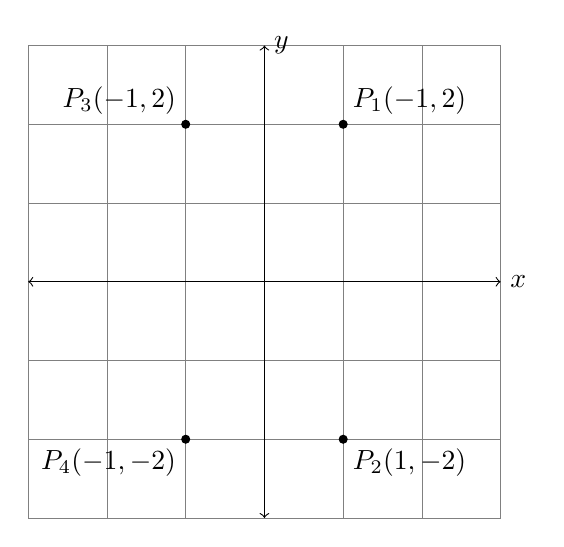
\begin{tikzpicture}
                \draw[step=1,gray,very thin] (-3,-3) grid (3,3);
                \draw[fill=black] (1,2) circle (0.05) node[above right] {$P_1(-1,2)$};
                \draw[fill=black] (1,-2) circle (0.05) node[below right] {$P_2(1,-2)$};
                \draw[fill=black] (-1,2) circle (0.05) node[above left] {$P_3(-1,2)$};
                \draw[fill=black] (-1,-2) circle (0.05) node[below left] {$P_4(-1,-2)$};
                \draw[<->] (-3,0) -- (3,0) node[right]{$x$};
                \draw[<->] (0,-3) -- (0,3) node[right]{$y$};

                \end{tikzpicture}
        \end{center}
        We can represent the four coordinates also as:
        \begin{align}
            P_1[\sqrt{5}, 1.107] \\ 
            P_2[\sqrt{5}, -1.107] \\ 
            P_3[-\sqrt{5}, -1.107] \\ 
            P_4[-\sqrt{5}, 1.107]
        \end{align}
    \end{example}
    \item We can represent straight lines as:
    \begin{itemize}
        \item Straight lines: $y=mx$: $r=\alpha$ with $\alpha=\arctan(m)$.
        \item Vertical lines $x=a$: We have $r\cos\theta = a \implies r = a\sec\theta$.
        \item Horizontal lines: $y=b$. We have $r\sin\theta=b \implies r=b\csc\theta$
    \end{itemize}
    \item We can represent circles in polar coordinates as:
    \begin{equation}
        x^2 + y^2 = 9 \iff r = 3
    \end{equation}
    \item Converting \textit{from} polar coordinates requires a bit of extra work. Suppose we have $r=6\sin\theta$, then:
    \begin{align}
        r^2 &= 6r\sin\theta \\ 
        x^2+y^2 &= 6y \\ 
        x^2+y^2-6y+9=9 \\ 
        x^2 + (y-3)^2 &= 9
    \end{align}
    which represents a circle with radius $3$ centered at $(0,3)$.
    \item Symmetry can also arise in many scenarios. For example:
    \begin{itemize}
        \item Symmetry about $x$ axis: $[r_1,\theta]$ and $[r_1, -\theta]$.
        \item Symmetry about $y$ axis: $[r, \pi-\theta]$ and $[r_1, \theta]$.
        \item Symmetry about origin: $[r,\theta]$ and $[r, \theta + \pi]$.
    \end{itemize}
    which will help when sketching them.
    \begin{example}
        Suppose we wish to sketch the curve $r= \frac{1}{2} + \cos\theta$. Notice that this is periodic so we only need to look at values of $\theta$ where $0 \le \theta < 2\pi$.
        \begin{enumerate}
            \item Let us first find values of $\theta$ (if possible) that make $r=0$:
            \begin{equation}
                0 = \frac{1}{2} + \cos\theta \implies \theta = \frac{2\pi}{3}, \frac{4\pi}{3}
            \end{equation}
            \item Find local max and min values of $r$:
            \begin{equation}
                \frac{dr}{d\theta} = -\sin\theta = 0 \implies \theta = 0, \pi
            \end{equation}
            At $\theta=0$, we have $r=\frac{3}{2}$, at $\theta= \pi$ we have $r = -\frac{1}{2}$. If $\theta = \frac{\pi}{2}, \frac{3\pi}{2}$, then $r=\frac{1}{2}$.
            \item We then loko at symmetry. Notice that:
            \begin{equation}
                \frac{1}{2} + \cos(-\theta) + \frac{1}{2}+\cos\theta
            \end{equation}
            However:
            \begin{align}
                r(\theta - \pi) \neq r(\theta) \\ 
                r(\pi + \theta) \neq r(\theta)
            \end{align}
            so it is not symmetryic about the $y$ axis or origin.
            \item We now look at the relevant intervals. From $0 \le \theta < \frac{2\pi}{3}$, we have $\frac{dr}{d\theta} < 0$ so the radius is monotonically decreasing.
            \vspace{2mm}

            We can also look at the interval $\frac{2\pi}{3} \le \theta < \pi$ and see that $r$ is negative and $\frac{dr}{d\theta} < 0$, so the manigutde of $r$ \textit{increases}.
            \vspace{2mm}

            Noting that the function is differentiable at $\theta=\pi$, we can reflect the shape about the $x$ axis to get a Limacon with inner loop.
        \end{enumerate}
    
    \begin{center}
        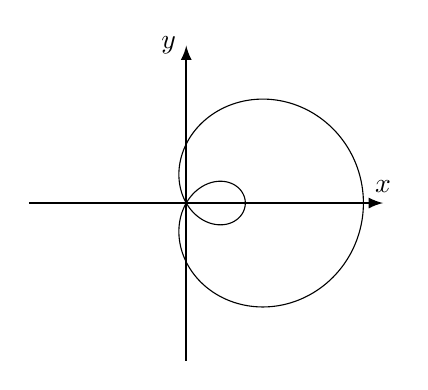
\begin{tikzpicture}
            \draw[thick,->,>=latex] (-2,0)--(2.5,0) node[above] {$x$};
            \draw[thick,->,>=latex] (0,-2)--(0,2) node[left] {$y$};
            \draw[domain=0:540,scale=1.5,samples=500] plot (\x:{0.5+cos(\x)});
        \end{tikzpicture}
    \end{center}
    \end{example}
    \item There are a few common shapes. Each of these could be flipped or rotated by shifting the argument $\theta$, or using negative numbers.
    \begin{itemize}
        \item Circles:
        \begin{equation}
            r = -2\cos\theta
        \end{equation}
        \begin{center}
            \begin{tikzpicture}
                \draw[thick,->,>=latex] (-3,0)--(3,0) node[above] {$x$};
                \draw[thick,->,>=latex] (0,-3)--(0,3) node[left] {$y$};
                \draw[domain=0:540,scale=1.5,samples=500] plot (\x:{-2*cos(\x)});
            \end{tikzpicture}
        \end{center}
        \item Cardioids:
        \begin{equation}
            r= a + a\cos\theta 
        \end{equation}

        \begin{center}
            \begin{tikzpicture}
                \draw[thick,->,>=latex] (-3,0)--(3,0) node[above] {$x$};
                \draw[thick,->,>=latex] (0,-3)--(0,3) node[left] {$y$};
                \draw[domain=0:540,scale=1.5,samples=500] plot (\x:{1+1*cos(\x)});
            \end{tikzpicture}
        \end{center}
        \item Limacons:
        \begin{equation}
            r=a+b\sin\theta
        \end{equation}
        There are two types, for $a>b$:
        \begin{center}
            \begin{tikzpicture}
                \draw[thick,->,>=latex] (-3,0)--(3,0) node[above] {$x$};
                \draw[thick,->,>=latex] (0,-3)--(0,3) node[left] {$y$};
                \draw[domain=0:540,scale=1.5,samples=500] plot (\x:{1+0.5*cos(\x)});
            \end{tikzpicture}
        \end{center}
        For $a<b$:
        \begin{center}
            \begin{tikzpicture}
                \draw[thick,->,>=latex] (-3,0)--(3,0) node[above] {$x$};
                \draw[thick,->,>=latex] (0,-3)--(0,3) node[left] {$y$};
                \draw[domain=0:540,scale=1.5,samples=500] plot (\x:{0.5+1*cos(\x)});
            \end{tikzpicture}
        \end{center}
        \item Leminiscates. Again, there are two types. For:
        \begin{equation}
            r^2 = a\sin(2\theta)
        \end{equation}
        \begin{center}
            \begin{tikzpicture}
                \draw[thick,->,>=latex] (-3,0)--(3,0) node[above] {$x$};
                \draw[thick,->,>=latex] (0,-3)--(0,3) node[left] {$y$};
                \draw[domain=0:90,scale=1.5,samples=500] plot (\x:{sqrt(sin(2*\x))});
                \draw[domain=0:90,scale=1.5,samples=500] plot (\x:{-sqrt(sin(2*\x))});
            \end{tikzpicture}
        \end{center}
        and:
        \begin{equation}
            r^2 = a\cos(2\theta)
        \end{equation}
        \begin{center}
            \begin{tikzpicture}
                \draw[thick,->,>=latex] (-3,0)--(3,0) node[above] {$x$};
                \draw[thick,->,>=latex] (0,-3)--(0,3) node[left] {$y$};
                \draw[domain=-45:45,scale=1.5,samples=500] plot (\x:{sqrt(cos(2*\x))});
                \draw[domain=-45:45,scale=1.5,samples=500] plot (\x:{-sqrt(cos(2*\x))});
            \end{tikzpicture}
        \end{center}
        \item Petal curves:
        \begin{align}
            r &= a\sin(n\theta) \\ 
            r &= a\cos(n\theta)
        \end{align}
        where $n$ is an integer. There are $n$ petals if $n$ is odd and $2n$ petals if $n$ is even. For example, the following is: $r=2\cos 3\theta$:
        \begin{center}
            \begin{tikzpicture}
                \draw[thick,->,>=latex] (-3,0)--(3,0) node[above] {$x$};
                \draw[thick,->,>=latex] (0,-3)--(0,3) node[left] {$y$};
                \draw[domain=0:360,scale=1.5,samples=500] plot (\x:{2*cos(3*\x)});
            \end{tikzpicture}
        \end{center}
        and for $r=2\sin(4\theta)$:
        \begin{center}
            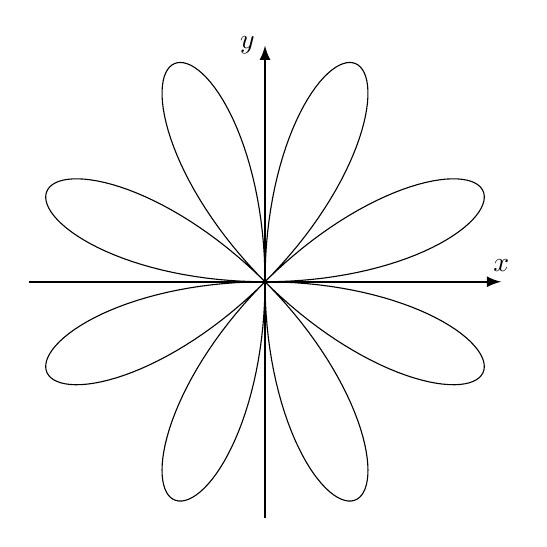
\begin{tikzpicture}
                \draw[thick,->,>=latex] (-3,0)--(3,0) node[above] {$x$};
                \draw[thick,->,>=latex] (0,-3)--(0,3) node[left] {$y$};
                \draw[domain=0:360,scale=1.5,samples=500] plot (\x:{2*sin(4*\x)});
            \end{tikzpicture}
        \end{center}
    \end{itemize}
    \item We can also find the intersection of polar coordinates, but we have to be careful. The following example illustrates why.
    \begin{example}
        Suppose we have two curves $r=\sin\theta$ and $r=-\cos\theta$. Suppose we try to solve this via:
        \begin{equation}
            \sin\theta = -\cos\theta \implies \theta = \frac{3\pi}{4}, \frac{7\pi}{4}
        \end{equation}
        Plugging this back into $x=r\cos\theta$ and $y=r\sin\theta$, we get $x=-\frac{1}{2}$ and $y=-\frac{1}{2}$. We can also use $\theta=\frac{7\pi}{4}$ to get: $x=-\frac{1}{2}$ and $y=\frac{1}{2}$ which is the same point. However, it represents the curves below:
        \begin{center}
            \begin{tikzpicture}
                \draw[thick,->,>=latex] (-3,0)--(3,0) node[above] {$x$};
                \draw[thick,->,>=latex] (0,-3)--(0,3) node[left] {$y$};
                \draw[domain=0:540,scale=1.5,samples=500] plot (\x:{-cos(\x)});
                \draw[domain=0:540,scale=1.5,samples=500] plot (\x:{sin(\x)});
            \end{tikzpicture}
        \end{center}
        There is actually two intersection points! The reason for this is that we assumed that the two curves intersect at the same value of $\theta$, but this is not necessarily true for the origin, which can be obtained at any angle $\theta$.
    \end{example}
    \item As a result, we also have to check the origin.
    \item It is also possible to find the tangent:
    \begin{align}
        \frac{dy}{dx} &= \frac{
            \frac{dy}{d\theta}
            }{
                \frac{dx}{d\theta}
            } \\ 
            &= \frac{
            \frac{dr}{d\theta} \sin\theta + r\cos\theta
            }{
                \frac{dr}{d\theta} \cos\theta - r\sin\theta
            }
    \end{align}
\end{itemize}
    % \section{Areas and Lengths in Polar Coordinates}
\begin{itemize}
    \item Suppose we have a polar curve $r= \rho(\theta)$ for $\alpha \le \theta \le \beta$.
    \item We can determine the area by partitioning the curve into $\theta_i$ and approximating each subregion as a circular segment. The area of a circular segment is:
    \begin{equation}
        A = \frac{1}{2}a^2\Delta \theta
    \end{equation}
    We can take the radius to be $r = \rho(\theta^*)$ where $\theta_{i-1} \le \theta^* \le \theta_i$. The area of each region is:
    \begin{equation}
        A_i = \frac{1}{2}\rho(\theta_i^*)^2 \Delta \theta_i
    \end{equation}
    so the total area is:
    \begin{equation}
        A = \lim_{|| P ||} \sum_{i} \frac{1}{2}\rho(\theta_i^*)^2 \Delta \theta_i
    \end{equation}
    or
    \begin{equation}
        A = \frac{1}{2} \int_\alpha^\beta \rho(\theta)^2 \dd{\theta}
    \end{equation}
    \begin{example}
        Suppose we wish to find the area of $r = 1 - \cos\theta$.
        \begin{center}
            \begin{tikzpicture}
                \draw[thick,->,>=latex] (-3,0)--(3,0) node[above] {$x$};
                \draw[thick,->,>=latex] (0,-3)--(0,3) node[left] {$y$};
                \draw[domain=0:360,scale=1.5,samples=500] plot (\x:{1-cos(\x)});
            \end{tikzpicture}
        \end{center}
        The area is then:
        \begin{align}
            A &= \frac{1}{2}\int_0^{2\pi} (1-\cos\theta)^2 \dd{\theta} \\ 
            &= \frac{1}{2}\int_0^{2\pi} (1-2\cos\theta+\cos^2\theta)\dd{\theta} \\ 
            &= \frac{1}{2}\int_0^{2\pi} \left(\frac{3}{2}-2\cos\theta + \frac{1}{2}\cos(2\theta)\right) \dd{\theta} \\ 
            &= \frac{1}{2}\left(\frac{3}{2}\theta - 2\sin\theta + \frac{1}{4}\sin(2\theta) \right)\Biggr|^{2\pi}_{0} \\ 
            &= \frac{3}{2}\pi
        \end{align}
    \end{example}
    \item We can also find the area between two polar curves $\rho_1$ and $\rho_2$. We have:
    \begin{equation}
        A = \frac{1}{2}\int_\alpha^\beta \rho_1(\theta)^2 \dd{\theta} - \frac{1}{2}\int_\alpha^\beta \rho_2(\theta)^2 \dd{\theta} = \frac{1}{2}\int_\alpha^\beta (\rho_1^2-\rho_2^2)\dd{\theta}
    \end{equation}
    \begin{warning}
        Be careful when applying this formula as it is possible the two functions can overlap between $\alpha \le \theta \le \beta$. Therefore, we always need a good idea of what's happening.
    \end{warning}
    \begin{example}
        Suppose we want to determine the area inside $r^2 = 4\cos(2\theta)$ but outside $r=1$. This gives:
        \begin{center}
            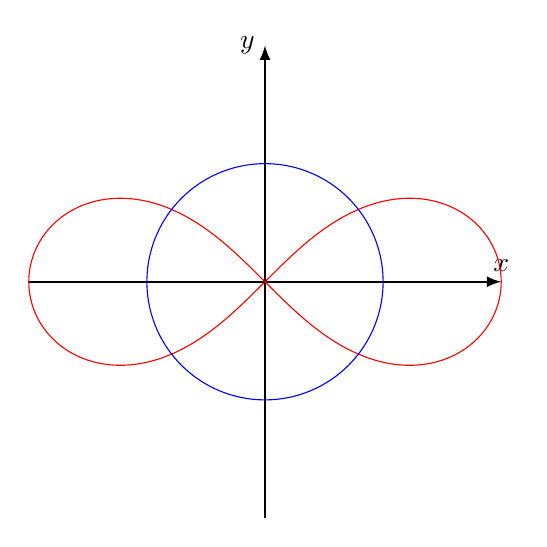
\begin{tikzpicture}
                \draw[thick,->,>=latex] (-3,0)--(3,0) node[above] {$x$};
                \draw[thick,->,>=latex] (0,-3)--(0,3) node[left] {$y$};
                \draw[red, domain=-45:45,scale=1.5,samples=500] plot (\x:{sqrt(4*cos(2*\x))});
                \draw[red, domain=-45:45,scale=1.5,samples=500] plot (\x:{-sqrt(4*cos(2*\x))});
                \draw[blue, domain=0:360,scale=1.5,samples=500] plot (\x:{1});
            \end{tikzpicture}
        \end{center}
        We first find the four points of intersection:
        \begin{equation}
            4\cos(2\theta)=1 \implies \cos (2\theta) = \frac{1}{4} \implies \theta = \pm 0.659
        \end{equation}
        or $\theta = \pi \pm 0.659$. Due to the symmetry, we only need to find the area of one half of the area we are interested in, which gives:
        \begin{align}
            \frac{1}{2}A &= \frac{1}{2}\int_{-0.659}^{0.659}(4\cos 2\theta - 1) \dd{\theta} \\ 
            &= \frac{1}{2}(2\sin 2\theta - \theta)\Big|^{0.659}_{-0.659} \\
            &= 1.277
        \end{align}
        so the area is $A=2.554$.
    \end{example}
    \item There are a few challenging examples:
    \begin{example}
        Suppose we wish to find the area between $r=\sin\theta$ and $r=\cos \theta$:
        \begin{center}
            \begin{tikzpicture}
                \draw[thick,->,>=latex] (-3,0)--(3,0) node[above] {$x$};
                \draw[thick,->,>=latex] (0,-3)--(0,3) node[left] {$y$};
                \draw[red, domain=0:360,scale=2.5,samples=500] plot (\x:{cos(\x)});
                \draw[blue, domain=0:360,scale=2.5,samples=500] plot (\x:{sin(\x)});
            \end{tikzpicture}
        \end{center}
        We know from symmetry that the intersection is at $\theta = \frac{\pi}{4}$. We notice that the contribution to the area from each curve $\rho$ is equal and \textit{independent} from each other. Therefore:
        \begin{equation}
            A = A_1 + A_2 = \int_0^{\pi/4} \frac{1}{2}\sin^2\theta \dd{\theta} + \int_{\pi/4}^{\pi/2} \frac{1}{2}\cos^2\theta \dd{\theta} = \frac{\pi}{8} - \frac{1}{4}
        \end{equation}
    \end{example}
    \item We can determine the arclength by working in parametric form. Let $x = r(\theta) \cos\theta$ and $y = r(\theta) \sin\theta$. Therefore:
    \begin{align}
        s &= \int_{\alpha}^{\beta} \sqrt{\left(\frac{dx}{d\theta}\right)^2 + \left(\frac{dy}{d\theta}\right)^2}\dd{\theta} \\ 
        &= \int_\alpha^\beta \sqrt{(r'\cos\theta - r\sin\theta)^2 + (r'\sin\theta + r\cos\theta)^2} \dd{\theta} \\ 
        &= \int_\alpha^\beta \sqrt{(r'^2\cos^2\theta + r^2\sin^2\theta - \cancel{2rr'\cos\theta\sin\theta}) + (r'^2\sin^2\theta + r^2\cos^2\theta + \cancel{2r'r\cos\theta\sin\theta})} \dd{\theta} \\ 
        &= \int_\alpha^\beta \sqrt{r^2(\cos^2\theta+\sin^2\theta) + r'^2(\cos^2\theta+\sin^2\theta)} \\ 
        &= \int_\alpha^\beta \sqrt{r^2 + \left(\frac{dr}{d\theta}\right)^2} \dd{\theta}
    \end{align}
    \begin{example}
        Suppose we want to find the arclength of $r=a(1-\cos\theta)$ from $0 \le \theta < 2\pi$. This looks like:
        \begin{center}
            \begin{tikzpicture}
                \draw[thick,->,>=latex] (-3,0)--(3,0) node[above] {$x$};
                \draw[thick,->,>=latex] (0,-3)--(0,3) node[left] {$y$};
                \draw[domain=0:360,scale=1.5,samples=500] plot (\x:{1-cos(\x)});
            \end{tikzpicture}
        \end{center}
        We have:
        \begin{align}
            s &= \int_0^{2\pi}\sqrt{r^2 + (r')^2} \dd{\theta} \\ 
            &= \int_0^{2\pi}\sqrt{a^2(1-2\cos\theta+\cos^2\theta)+a^2\sin^2\theta}\dd{\theta} \\ 
            &= a\int_0^{2\pi}\sqrt{2-2\cos\theta}\dd{\theta} \\ 
            &= a \int_0^{2\pi} \sqrt{4\sin^2\left(\frac{\theta}{2}\right)} \dd{\theta} \\ 
            &= 2a\left[-2\cos\left(\frac{\theta}{2}\right)\right]\Biggr|^{2\pi}_0 \\ 
            &= 8a
        \end{align}
    \end{example}
\end{itemize}
    % \section{Lecture 13}
\begin{itemize}
    \item We introduce the \textbf{Mean Value Theorem (MVT)}. First, we need to prove a simpler version known as \textbf{Rolle's Theorem}
    \begin{theorem}
        Given that $f$ is continuous on $[a,b]$ and $f$ is differentiable on $[a,b)$ and $f(a)=f(b)$. Then there exists some $c \in (a,b)$ such that $f'(c)=0$. Note that there may be more than one $c$
    \end{theorem}
    \begin{prooof}
        There are only three possibilities:
        \begin{enumerate}
            \item $f(x)>f(a)$ for some $x$ in $(a,b)$
            \item $f(x)<f(a)$ for some $x$ in $(a,b)$
            \item $f(x)=f(a)=f(b)$ for all $x$ in $(a,b)$
        \end{enumerate}
        To prove the third case, since $f'(x)=0$ (C.D.T.), for all $x$ in $[a,b]$, then it is automatically satisfied. To prove the first case, by the extreme value theorem, there is an absolute maximum in $[a,b]$. It can't be an end-point maximum so it by Fermat's principle it must be a critical point. It can't be a critical point where the derivative doesn't exist, so it must be a point where $f'(c_\text{crit})=0$. The second case is identical to the first.
    \end{prooof}
    \begin{theorem}
        The \textbf{Mean Value Theorem:} Given that $f(x)$ is continuous on $[a,b]$ and $f(x)$ is differentiable on $(a,b)$, then there exists some $c\in (a,b)$ such that:
        \begin{equation}
            f'(c)=\frac{f(b)-f(a)}{b-a}
            \label{eq:}
        \end{equation}
        Note that both continuity and differentiability is needed.
    \end{theorem}
    \begin{example}
        Physics example: Let $d(t)$ be the distance travelled in time $t$. The $MVT$ tells us that at some time in the trip your instantaneous speed must equal your average speed on the trip.
    \end{example}
    \begin{prooof}
        The equation of a secant line is:
        \begin{equation}
            y_\text{secant}(x)=f(a)+\frac{f(b)-f(a)}{b-a}\left(x-a\right)
            \label{eq:13-secant}
        \end{equation}
        Note that this is in the form of $y_\text{secant}(x)=A+Bx$, a first order polynomial. Then we can define:
        \begin{equation}
            g(x)\equiv f(x)-y_\text{secant}(x)
            \label{eq:}
        \end{equation}
        We now show that $g(x)$ satisfies Rolle's theorem. $g(x)$ is continuous on $[a,b]$ since $f(x)$ is. Also $y_\text{secant}(x)$ is continuous (Poly CT) so $g(x)$ is also continuous (ACT). Similarly, $g(x)$ is also differentiable on $(a,b)$ since $f(x)$ is. $y_\text{secant}(x)$ is also differentiable per Poly DT and $g(x)$ is also (ADT). We have $g(a)=g(b)=0$, so by Rolle, there is some $c\in (a,b)$ such that $g'(c)=0$ or:
        \begin{equation}
            f'(c)-y_\text{secant}'(c)=0
            \label{eq:}
        \end{equation}
        Using equation \ref{eq:13-secant}, we have:
        \begin{equation}
            f'(c)=\frac{f(b)-f(a)}{b-a}
            \label{eq:}
        \end{equation}
    \end{prooof}
    \begin{example}
        Given $f(x)=x^2$ on $[2,3]$. Prove that $f$ satisfies the conditions of MVT. We have $f(a)=$ and $f(b)=9$ such that:
        \begin{equation}
            \frac{f(b)-f(a)}{b-a}=\frac{9-4}{3-2}=5
            \label{eq:}
        \end{equation}
        Is there some $c\in (2,3)$ such that $f'(c)=5$? Yes! We can let $f'(x)=2x=5 \implies x-5/2$. Since $2<5/2<3$, then this all checks out.
    \end{example}
\begin{multicols}{2}
    \textbf{General Case:}
    \begin{itemize}
        \item Let $y=f(x)$ where $y$ is the dependent variable and $x$ is the independent variable.
        \item Define increments $\Delta y$ and $\Delta x$, 2 \textit{new} variables! They are related by:
        \begin{equation}
            \Delta y = f(x+\Delta x)-f(x)
            \label{eq:}
        \end{equation}
        Here $\Delta x$ is the independent variable and $\Delta y$ is the dependent variable.
    \end{itemize}
    \vfill\null
    \columnbreak
    \textbf{Example Case:}
    \begin{itemize}
        \item Let $y=x^{1/3}$. Choose $x=27$ for example. We have free choice for picking the value of $x$.
        \item Choose $\Delta x=2$, say for example. Remember we have free choice! Then:
        \begin{equation}
            \Delta y = 29^{1/3}-27^{1/3}=29^{1/3}-3
            \label{eq:}
        \end{equation}
    \end{itemize}
\end{multicols}
\begin{idea}
    Note that the value of $\Delta y$ depends on choices for both $x$ and $\Delta x$!
\end{idea}
\begin{multicols}{2}
    \begin{itemize}
        \item Define differentials $dx$, $dy$, 2 new variables related by:
        \begin{equation}
            dy \equiv f'(x) dx
            \label{eq:}
        \end{equation}
    \end{itemize}
    \vfill\null
    \columnbreak
    \begin{itemize}
        \item Choose $dx=1/2$ for example. Then we can say:
        \begin{equation}
            dy=\underbrace{\frac{1}{3}(26)^{-2/3}}_\text{derivative of f}\left(\frac{1}{2}\right)=\frac{1}{54}
            \label{eq:}
        \end{equation}
    \end{itemize}
\end{multicols}
\begin{idea}
    Since $dx$ and $\Delta x$ are both independent variables, we are free to choose them to be equal: $dx=\Delta x$. This can be useful! Note that this implies that:
    \begin{equation}
        \Delta y \approx dy
        \label{eq:}
    \end{equation}
    is an approximation, and this approximation improves as $\Delta x \to 0$. The practical point is that we may want to know $\Delta y$, i.e. $f(x+\Delta x)-f(x)$. It may, however might be easy to calculate $f'(x)$ such that:
    \begin{equation}
        f(x+\Delta x) \approx f(x)+f'(x)\Delta x
        \label{eq:}
    \end{equation}
\end{idea}
\begin{example}
    Suppose we wish to estimate $29^{1/3}$, then we can define $f(x)=x^{1/3}$ and pick $x=27$, $\Delta x=2$ such that:
    \begin{align}
        \Delta y &= f(x+\Delta x)-f(x) \\ 
        &= f(29)-f(27)=29^{1/3}-3 
        \label{eq:}
    \end{align}
    We can now use the approximation $\Delta y \approx dy = f'(x)dx = f(x)\Delta x$ where:
    \begin{equation}
        \Delta y \approx \frac{1}{3}x^{-2/3}\Delta x = \frac{2}{27}
        \label{eq:}
    \end{equation}
    and:
    \begin{equation}
        \frac{2}{27} \approx 29^{1/3}-3 \implies 29^{1/3} \approx 3+\frac{2}{27}
        \label{eq:}
    \end{equation}    
\end{example}
\end{itemize}

    % \section{Lecture 14}
\begin{itemize}
    \item Using differentials, we estimated $29^{1/3} \approx 3.074$. We need to know how far it could be off.
    \item We can use the MVT to bracket our estimate. Apply the MVT to $f(x)=x^{1/3}$ on $[27,29]$. There is some $c \in (27,29)$ such that:
    \begin{equation}
        f'(c)=\frac{29^{1/3}-27^{1/3}}{29-27}=\frac{29^{1/3}-3}{2}
        \label{eq:}
    \end{equation}
    or:
    \begin{equation}
        f'(c)=\frac{1}{3}c^{-2/3}
        \label{eq:}
    \end{equation}
    Therefore:
    \begin{equation}
        29^{1/3}=3+\frac{2}{3}c^{-2/3}
        \label{eq:}
    \end{equation}
    The largest is when $c=27 \implies c^{-2/3}=\frac{1}{9}$. The smallest is when $c=29$, but we don't know what $29^{-2/3}$ is!
    \item Note however that $29<64$ such that:
    \begin{equation}
        29^{2/3} < 64^{2/3} = 16 \implies \frac{1}{16} < 29^{-2/3} \implies c^{-2/3} > \frac{1}{16}
        \label{eq:}
    \end{equation}
    and therefore:
    \begin{equation}
        3+\frac{2}{3}\frac{1}{16} < 29^{1/3} < 3+\frac{2}{3}\frac{1}{9} \implies 3.0416 < 29^{1/3} < 3.074
        \label{eq:}
    \end{equation}
    \item To graph functions, we need a few quick tests.
    \item QT1: First is the \textbf{Increasing/Decreasing Test}
    \begin{idea}
        Given that $f$ is differentiable on interval $I$, we show that:
    \begin{itemize}
        \item If $f'>0$, $f$ is increasing.
        \item If $f'<0$, $f$ is decreasing.
        \item If $f'=0$, $f$ is constant.
    \end{itemize}
    \end{idea}
    We can prove the first statement.
    \begin{proof}
        Since $f$ is differentiable, the MVT holds. There is some $c\ in I$ such that:
        \begin{equation}
            f(x_2)-f(x_1)= f'(c)(x_2-x_1) \implies f(x_2)-f(x_1)
            \label{eq:}
        \end{equation}
        which is the definition of an increasing function. The proof goes similarly for the other two.
    \end{proof}
    \item QT2: First derivative test. The motivation behind this is that $f(c_\text{crit})$ includes max and min values, but also others. How do we know which to keep?
    \begin{idea}
        Given that $I$ contains a critical point and $f$ is continuous at $c_\text{crit}$. $f$ is differentiable in $I$, but not necessarily at $c_\text{crit}$. Then:
        \begin{itemize}
            \item If $f'>0$ to the left of $c_\text{crit}$ and $f'<0$ is to the right, then $c_\text{crit}$ is a local max.
            \item If it's the opposite, we get the local minimum.
        \end{itemize}
    \end{idea}
    We can also prove this:
    \begin{proof}
        There is some $a$ such that $f'>0$ for $x \in (a,c)$, by QT1, $f$ is increasing where:
        \begin{equation}
            f(c) \ge f(x)
            \label{eq:}
        \end{equation}
        in $(a,c)$. There is also some $b$ such that $f'<0$ for $x \in (c,b)$ where $f'<0$. By QT1, $f$ decreases. As a result:
        \begin{equation}
            f(c) \ge f(x)
            \label{eq:}
        \end{equation}
        in $(c,b)$. Therefore:
        \begin{equation}
            f(c) \ge f(x)
            \label{eq:}
        \end{equation}
        for all $x\in (a,b)$. Therefore, $f(c)$ is a local maximum, by definition. 
    \end{proof}
    \item Concavity: Points of Inflection
    \begin{definition}
        If the graph of $y=f(x)$ lies above all its tangents in $I$, then $f(x)$ is concave up in $I$.
    \end{definition}
    \item QT3: Concavity Test:
    \begin{idea}
        Given that $f(x)$ is twice differentiable on $I$, then $f''(x)$ exists on $I$. As a result:
        \begin{itemize}
            \item If $f''>0$, $f$ is concave up.
            \item If $f''<0$, $f$ is concave down.
        \end{itemize}
    \end{idea}
    \begin{proof}
        Proof assigned (pg A43). Uses MVT and QT1.
    \end{proof}
    \begin{definition}
        A point of inflection is at $c$ if:
        \begin{itemize}
            \item $f(x)$ is continuous at $c$ and
            \item Sign of concavity changes at $c$.
        \end{itemize} 
    \end{definition}
    \begin{example}
        Let $f(x)=x^3$. Then $f'=3x^2$ and $f''=6x$. Since $f(x)$ is continuous at $c$ and the sign of concavity changes at $x=0$, therefore $(0,0)$ is an inflection point.
    \end{example}
    \item QT4: Second derivative test:
    \begin{idea}
        Given that $f''(x)$ is continuous near $c$ and $f'(c)=0$, then:
        \begin{itemize}
            \item If $f''(c)>0$, $f(c)$ is a local minimum.
            \item If $f''(c)<0$, $f(c)$ is a local maximum.
            \item If $f''(c)=0$, there is no verdict!
        \end{itemize}
    \end{idea}
    Note that this is even quicker than QT2!
    \begin{idea}
        In summary, the recipe to test for local max and min is to:
        \begin{itemize}
            \item Find all $c_\text{crit}$.
            \item If QT4 applies, use it.
            \item If it doesn't, and if QT2 applies, use it.
            \item If QT2 doesn't apply, use the basic definition of increasing/decreasing.
        \end{itemize}
    \end{idea}
\end{itemize}
    % \section{Lecture 15}
\begin{itemize}
    \item We can define horizontal asymptotes:
    \begin{definition}
        A horizontal asymptote occurs when $\lim_{x\to\infty}f(x)=L$. We can say that 
        $f(x)$ goes to $L$ as $x$ goes to infinity if for any $\epsilon>0$, a number $A$ can be found s.t. for all $x>A$, $|f(x)-L|<\epsilon$.
        \vspace{2mm}

        The idea behind this revolves around finding $f$ values as close to $L$ as might be wanted by going to large enough $x$ values.
    \end{definition}
    \item Geometrically, we can say that if $\displaystyle \lim_{x\to\infty}f(x) = L$, then the line $y=L$ is the horizontal asymptote of $f(x)$ at $x=\infty$.
    \begin{theorem}
        The reciprocal horizontal asymptote limit:
        \begin{equation}
            \lim_{x\to \pm \infty} \frac{1}{x^r} = 0
            \label{eq:}
        \end{equation}
    \end{theorem}
    \item Slant asymptotes are a thing too. For example, suppose we have the function:
    \begin{equation}
        f(x)=\frac{x+2}{1+\frac{1}{x^2}}
        \label{eq:}
    \end{equation}
    We might say that intuitively $f(x)\to x+2$ as $x\to \infty$.
    \begin{definition}
        If $\lim_{x\to \infty} \left[f(x)-(mx+b)\right]=0$, then $y=mx+b$ is a slant asymptote to $f(x)$ at $+\infty$.
    \end{definition}
    \item Curve Sketching Check-list:
    \begin{itemize}
        \item Find domain/range/limits at infinity, end points if they exist, vert/horz/slant asymptote
        \item Intercepts: Find x/y intercepts.
        \item Establish if $f(x)$ is symmetrical/even/odd/periodic
        \item Find $f'(x)$ then find all critical points and $f(c_\text{crit})$. Find when $f(x)$ is increasing/decreasing. Use 1st derivative test (QT2). Find vertical tangents/cusps if they exist.
        \item Find $f''(x)$, find where $f(x)$ is concave up/down. Find points of inflection if they exist. (Optional: use 2nd derivative test QT4 to confirm local max/min)
        \item Choose largest and smallest values of $f$ from the above as abs. max, min, if they exist.
    \end{itemize}
\end{itemize}
    % \section{Convergence Tests}
\begin{itemize}
    \item We start with the integral test:
    \begin{theorem}
        If $f$ is continuous, decreasing, and positive on $[1,\infty)$, then: $\sum_{k=1}^\infty f(k)$ converges if and only if $\int_1^\infty f(x) \dd{x}$ converges.
    \end{theorem}
    \begin{example}
        Suppose we take the harmonic sum:
        \begin{equation}
            \sum_{k=1}^\infty \frac{1}{k} = 1 + \frac{1}{2} + \frac{1}{3} + \frac{1}{4}
        \end{equation}
        However, the integral $\int_1^\infty \frac{\dd{x}}{x} = \lim_{b\to\infty} \ln b$ diverges.
    \end{example}
    \item The $p$-series is:
    \begin{equation}
        \sum_{k=1}^\infty \frac{1}{k^p}
    \end{equation}
    which will converge if $p > 1$ since $\int_1^\infty \frac{\dd{x}}{x^p}$ converges iff $p>1$.
    \begin{example}
        Suppose we wish to look at $\sum_{n=5}^\infty \frac{1}{n^2+9}$. First, we notice that:
        \begin{equation}
            \lim_{t\to\infty} \int_5^t \frac{\dd{x}}{x^2+9} = \lim_{t\to\infty} \left[\frac{1}{3}\tan^{-1}\left(\frac{x}{3}\right)\right]\Biggr|^{t}_5
        \end{equation}
        which converges, and after checking the relevant conditions, this means that the sum converges too.
    \end{example}
    \begin{definition}
        The \textbf{remainder} for a sequence $\{f_n\}$ is given as:
        \begin{equation}
            R_n = f(n) - f_n
        \end{equation}
        where $f(n)$ denotes a continuous functoin while $f_n$ is discrete.
    \end{definition}
    \item For a decreasing function, $R_n \le \int_{n}^\infty f(x) \dd{x}$ and $R_n \ge \int_{n+1}^\infty f(x) \dd{x}$. This means that:
    \begin{equation}
        S_n + \int_{n+1}^\infty f(x) \dd{x} \le S \le S_n + \int_n^{\infty} f(x) \dd{x}
    \end{equation}
    \item We can also use the \textbf{comparison test}
    \begin{theorem}
        Given $\sum a_k$ and $\sum b_k$ with $a_k > 0 $ and $b_k > 0$:
        \begin{enumerate}
            \item If $\sum b_k$ is convergent, and if $a_k \le b_k$ for all sufficiently large $k$, then $\sum a_k$ converges.
            \item If $\sum b_k$ is diverge and $a_k > b_k$ for all $k$ sufficiently large, then $\sum a_k$ diverges.
        \end{enumerate}
    \end{theorem}
    \begin{proof}
        Assume $a_k \le b_k$ for all $k$ we can define:
        \begin{equation}
            S_n = \sum_{k=1}^n a_k
        \end{equation}
        as the sequence of partial sums where:
        \begin{equation}
            b_k = \sum_{k=1}^n b_k
        \end{equation}
        where $t=\sum_{k=1}^\infty b_k$ exists. This implies that $\{S_n\}$ is increasing since $a_k > 0$ and so:
        \begin{equation}
            S_n \le t_n < t
        \end{equation}
        where $\{S_n\}$ is a bounded sequence. By the monotonic sequence theorem, $\{S_n\}$ has a limit and $\sum_{k=1}^\infty a_k$ is defined to be equal to that limit. Therefore, $\sum a_k$ converges.
    \end{proof}
    \begin{example}
        Suppose we wish to determine if $\sum_{n=1}^\infty \frac{7}{17n^2+3\sqrt{n}+5}$ converges. Notice that for $n \ge 1$, we have:
        \begin{equation}
            17n^2+3\sqrt{n}+5 > 17n^2
        \end{equation}
        and so:
        \begin{equation}
            \frac{7}{17n^2+3\sqrt{n}+5} < \frac{7}{17n^2}
        \end{equation}
        Since $\frac{7}{17}\sum \frac{1}{n^2}$ converges, then the original sum must also converge.
    \end{example}
    \begin{example}
        Suppose we wish to determine if $\sum_{k=1}^\infty \frac{\ln(n/1000)}{n}$ converges. We want to find a $k$ such that:
        \begin{equation}
            \frac{\ln(k/1000)}{k} > \frac{1}{k}
        \end{equation}
        wihch means that we want to pick $k > 1000e > 2718$. Therefore, since $\sum_{k=2719}^\infty \frac{1}{k}$ is divergent, then the original sum is also divergent.
    \end{example}
    \item Suppose we wish to determine if $\sum{n=2}^\infty$ converges. This looks like $\frac{1}{n^3}$, but we notice that:
        \begin{equation}
            \frac{1}{n^3-n} > \frac{1}{n^3}
        \end{equation}
        and we run into trouble. This means we have to turn to the \textbf{limit comparison test}
    \begin{theorem}
        The limit comparison test: Given $\sum a_k$, $\sum b_k$ where $a_k > 0 $ and $b_k > 0$:
        \begin{enumerate}
            \item If $\lim_{n\to\infty} \frac{a_n}{b_n} = c > 0$, then both series converge or diverge.
            \item If $\lim_{n\to\infty} \frac{a_n}{b_n} = 0$ and if $\sum b_{n}$ converges, then $\sum_{a_n}$ converges.
            \item If $\lim_{n\to\infty} \frac{a_n}{b_n} = \infty$ and if $\sum b_n$ diverges, then $\sum a_n$ diverges.
        \end{enumerate}
    \end{theorem}
    \begin{proof}
        We are given that:
        \begin{equation}
            \lim_{n\to\infty} \frac{a_n}{b_n} = c \implies \left|\frac{a_n}{b_n}-c\right| < \epsilon
        \end{equation}
        for $n<N$. We are working \textit{backwards} here, so we are free to choose \textit{any} value of $\epsilon$ and this will hold true. We can choose $\epsilon = \frac{c}{2}$ such that:
        \begin{equation}
            \frac{c}{2} < \frac{a_n}{b_n} < \frac{3c}{2}
        \end{equation}
        which gives:
        \begin{equation}
            \frac{c}{2}b_n < a_n < \frac{3c}{2}b_n
        \end{equation}
        with $n>N$. If $\sum b_n$ converges, so does $\frac{3c}{2}\sum b_n$ since $c$ is just a number. Thereforfe, $\sum a_n$ converges by the comparison test. If $\sum b_n$ diverges, so does $\frac{c}{2}\sum b_n$ and again by the comparison test, $\sum a_n$ diverges.
    \end{proof}
    \begin{example}
        We continue our previous discussion of $\sum_{n=2}^\infty \frac{1}{n^3-n}$. We let $a_n = \frac{1}{n^3-n}$ and $b_n= \frac{1}{n^3}$. Both $a_n$ and $b_n$ are convergent and:
        \begin{equation}
            \lim_{n\to\infty} \frac{a_n}{b_n} = \lim_{n\to\infty} \frac{1}{1-\frac{1}{n^2}}=1 > 0
        \end{equation}
        so the original sequence is convergent.
    \end{example}
    \begin{example}
        We can also revisit $\sum \frac{\ln(n/1000)}{n}$. We consider $a_n = \frac{\ln(n/1000)}{n}$ and $b_n=\frac{1}{n}$. Since $\sum b_n$ diverges and $\lim_{n\to\infty} \frac{a_n}{b_n}$ diverges too, then $\sum a_n$ diverges as well.
    \end{example}
\end{itemize}
    \section{Lecture 17: Sigma Notation + Areas}
\begin{itemize}
    \item We begin by introducing sigma notation:
    \begin{definition}
        If $a_m,a_{m+1},a_{m+2},\dots,a_n$ are real numbers and $m$ and $n$ are integers such that $m\le n$, then:
        \begin{equation}
            \sum_{i=m}^{n}a_i=a_m+a_{m+1}+\cdots+a_{n-1}+a_n
            \label{eq:}
        \end{equation}
    \end{definition}
    For example:
    \begin{equation}
        \sum_{i=1}^4 i^2 = 1^2+2^2+3^3+4^2
        \label{eq:}
    \end{equation}
    There are a few theorems:
    \begin{itemize}
        \item For a constant $\alpha$:
        \begin{equation}
            \sum_{i=m}^n \alpha a_i = \alpha\sum_{i=m}^n a_i
            \label{eq:}
        \end{equation}
        \item It is also linear:
        \begin{equation}
            \sum_{i=m}^n (a_i+b_i) = \sum_{i=m}^na_i + \sum_{i=m}^nb_i
            \label{eq:}
        \end{equation}
        \item $\sum_{i=1}^n \alpha = \alpha n$
        \item $\sum_{i=1}^n i = \frac{n(n+1)}{2}$
        \item $\sum_{i=1}^n i^2 = \frac{n(n+1)(2n+1)}{6}$
        \item $\sum_{i=1}^n i^3 = \left(\frac{n(n+1)}{2}\right)^2$
        \item $\sum_{i=1}^n i^4 = \frac{n(n+1)(2n+1)(3n^2+3n-1)}{30}$
    \end{itemize}
    \item We can prove the last few properties via \textbf{induction}.
    \item We can also have limits inducing sums. For example, we can think of a sum as a function of $n$:
    \begin{equation}
        \sum_{i=1}^n a_i = f(n)
        \label{eq:}
    \end{equation}
    We can then think of the limit:
    \begin{equation}
        \lim_{n\to\infty}\sum_{i=1}^na_i
        \label{eq:}
    \end{equation}
    Since $n$ is a parameter, it can appear in other parts of the sum as well.
    \begin{example}
        Evaluate $\lim_{n\to \infty}\left[\frac{5}{n}\sum_{i=1}^n\left(\frac{i}{n}\right)^2\right]$. We can evaluate this by separating: to get:
        \begin{align}
            \lim_{n\to \infty}\left[\frac{5}{n}\sum_{i=1}^n\left(\frac{i}{n}\right)^2\right] &= \lim_{n\to\infty} \left(\frac{5}{n^3}\sum_{i=1}^n i^2\right) \\ 
            &= \lim_{n\to\infty} \left(\frac{5}{n^3}\frac{n(n+1)(2n+1)}{6}\right) \\ 
            \frac{5}{3}
        \end{align}
    \end{example}
    \item Suppose we wish to solve the problem of determining the area under a curve. We can do this via a Riemann sum by approximating a curve as many sub-intervals.
    \begin{example}
        Suppose we wish to find the area under the curve of $x \in [0,1]$. Then if there are $n$ rectangles, then the width of each rectangle is
        \begin{equation}
            \text{width} = \frac{1-0}{n}=\frac{1}{n}
            \label{eq:}
        \end{equation}
        The height for each of these is:
        \begin{equation}
            \frac{1}{n^2},\frac{2^2}{n^2},\dots,\frac{n^2}{n^2}
            \label{eq:}
        \end{equation}
        so the total area is:
        \begin{align}
            \text{Area} &= \frac{1}{n}\frac{1}{n^2}+\frac{1}{n}\frac{2^2}{n^3}+\cdots+\frac{1}{n}\frac{n^2}{n^2} \\ 
            &= \frac{1}{n^3}(1+2^2+3^2+\cdots+n^2) \\ 
            &= \frac{1}{n^3}\sum_{i=1}^n i^2 \\ 
            &= \frac{n(n+1)(2n+1)}{6n^3} \\
            &= \frac{(n+1)(2n+1)}{6n^2} \\
        \end{align}
        We can take the limit to find the area to be $\text{Area}=\frac{1}{3}.$
    \end{example}
    \begin{definition}
        A partition is a finite subset of the closed interval $[a,b]$, which contains the points $a$ and $b$. Denoted by $P$.
    \end{definition}
    \begin{definition}
        The norm of $P=\lVert P \rVert$ which is the length of the longest subinterval:
        \begin{equation}
            \lVert P \rVert = \max\left(\Delta x_1, \Delta x_2, \dots , \Delta x_n\right)
        \end{equation}
    \end{definition}
    \item In general, the approximated total area under a curve becomes:
    \begin{equation}
        \sum_{i=1}^n A_i = \sum_{i=1}^n f(x_i^*)\Delta x_2
    \end{equation}
    And we let the largest subinterval go to zero:
    \begin{equation}
        A = \lim_{\lVert P \rVert \to 0} \sum_{i=1}^n f(x_i^*)\Delta x_i
        \label{eq:}
    \end{equation}
    to get the total area.
    \begin{idea}
        In practice, our subintervals would be equal but this is not always the case in numerical methods.
    \end{idea}
    \begin{example}
        Let $y=\cos x$ and $0\le x\le b\le \frac{\pi}{2}$. To find the area, we can choose a regular partition:
        \begin{equation}
            \Delta x_1= \Delta x_2 = \dots = \Delta x_n = \frac{b}{n} = \lVert P \rVert
            \label{eq:}
        \end{equation}
        The right hand endpoints are:
        \begin{equation}
            x_i^*=x_i=\frac{ib}{n}
            \label{eq:}
        \end{equation}
        The area is thus:
        \begin{align}
            A &= \lim_{\lVert P \rVert \to 0} \sum_{i=1}^n f(x_i^*)\Delta x_i \\ 
            &= \lim_{n\to \infty}\sum_{i=1}^n \cos\left(\frac{ib}{n}\right)\cdot \frac{b}{n}
            \label{eq:}
        \end{align}
        We can apply the identity that:
        \begin{equation}
            \sum_{i=1}^n \cos(ix) = \frac{\sin(nx/2)\cos\left(\frac{x}{2}(n+1)\right)}{\sin(x/2)}
            \label{eq:}
        \end{equation}
        If we let $x=\frac{b}{n}$, then we get:
        \begin{align}
            A &= \lim_{n\to \infty} \frac{b}{n} \frac{\sin(b/2)\cos\left(\frac{(n+1)b}{2n}\right)}{\sin(b/2n)} 
        \end{align}
        We can look at the limit involving the cosine term:
        \begin{align}
            \lim_{n\to \infty} \cos\left(\frac{(n+1)n}{2n}\right) = \cos\left(\frac{b}{2}\right)
        \end{align}
        We can then make the substitution $t=\frac{b}{2n}$ to get:
        \begin{align}
            \lim_{n\to \infty} \frac{b}{2n} \cdot \frac{2}{\sin(b/2m)} &= \lim_{t\to 0+} 2\cdot \frac{t}{\sin t} \\ 
            &= 2
        \end{align}
        Similarly, we can find the limit of the denominator to get:
        \begin{equation}
            A = 2\sin(b/2)\cos(b/2)=\sin(b)
            \label{eq:}
        \end{equation}
    \end{example}
    \item Here is an example using a nonuniform partition.
    \begin{example}
        Evaluate $\int_0^2 x^{1/2} dx$. We can use a non-uniform partition:
        \begin{equation}
            x_i=i^2\frac{2}{n^2}
            \label{eq:}
        \end{equation}
        such that:
        \begin{equation}
            \Delta x_i=x_i-x_{i-1} = \frac{2}{n^2}\left(i^2-(i-1)^2\right)
            \label{eq:}
        \end{equation}
        For example for $n=4$:
        \begin{equation}
            P=\left\{0,\frac{2}{16},\frac{8}{16},\frac{18}{16},\frac{32}{16}\right\}
            \label{eq:}
        \end{equation}
        We can then approximate the area as:
        \begin{align}
            A &\approx \sum_{i=1}^n \Delta x_i f(x_i) \\ 
            &= \sum_{i=1}^n \frac{2}{n^2}\left(i^2-(i-1)^2\right) \cdot \left(i^2 \frac{2}{n^2}\right)^{1/2} \\
            &= \sum_{i=1}^n \frac{2\sqrt{2}}{n^3}(i(i^3-i^2+2i-1)) \\ 
            &= \sum_{i=1}^n \frac{2\sqrt{2}}{n^3}(2i^2-1) \\ 
            &= \frac{2\sqrt{2}}{3} \left(2+\frac{3}{n}+\frac{1}{n^2}\right)
            \label{eq:}
        \end{align}
        where we have applied our properties. Taking the limit as $n\to\infty$ gives us:
        \begin{equation}
            A = \frac{2}{3}2^{3/2}
            \label{eq:}
        \end{equation}
        Note that we also have to check that each of our subintervals go to zero, or:
        \begin{equation}
            \lim_{n\to \infty} \lVert P \rVert = \Delta x_n = \frac{2}{n^2}\left(n^2-(n-1)^2\right) = 0
            \label{eq:}
        \end{equation}
        
    \end{example}
\end{itemize}
    \end{document}